\documentclass{book}
\usepackage{html}
\usepackage{fancyhdr}
\usepackage{graphicx}

\newcommand{\gnutls}{{\emph{GNUTLS}}} 
\newcommand{\tlsI}{{\emph{TLS 1.0}}} 
\newcommand{\tls}{{\emph{TLS}}} 
\newcommand{\sslIII}{{\emph{SSL 3.0}}} 
\newcommand{\sslII}{{\emph{SSL 2.0}}} 
\newcommand{\ssl}{{\emph{SSL}}} 
\newcommand{\HRule}{\rule{\linewidth}{0.4mm}}


\begin{document}

\pagenumbering{roman}

\thispagestyle{empty}

\begin{quotation}
This document includes text contributed by
Nikos Mavrogiannopoulos, Simon Josefsson, Daiki Ueno, 
Carolin Latze, Alfredo Pironti, Ted Zlatanov and Andrew McDonald. Several corrections are due
to Patrick Pelletier and Andreas Metzler.
\end{quotation}

\vspace*{\stretch{2}}


\begin{flushleft}
ISBN 978-1-326-00266-4\\
Copyright \copyright{} 2001-2015 Free Software Foundation, Inc.\\
Copyright \copyright{} 2001-2015 Nikos Mavrogiannopoulos
\end{flushleft}

\begin{flushleft}
Permission is granted to copy, distribute and/or modify this document
under the terms of the GNU Free Documentation License, Version 1.3 or
any later version published by the Free Software Foundation; with no
Invariant Sections, no Front-Cover Texts, and no Back-Cover Texts.  A
copy of the license is included in the section entitled ``GNU Free
Documentation License''.
\end{flushleft}

\newpage
\thispagestyle{empty}

\vspace*{\stretch{2}}
\begin{center}

\includegraphics[width=6cm]{../gnutls-logo.pdf}
\end{center}

\vspace*{\stretch{2}}


\tableofcontents
\newpage
\pagenumbering{arabic}
\pagestyle{fancy}
\fancyhead[RE]{\slshape \rightmark}
\fancyhead[LO]{\slshape \leftmark}
\fancyhead[RO,LE]{\empty}
\fancyfoot[C]{\thepage}

\chapter{The Library}
\section{Introduction}
\par
\gnutls{} is a portable library which implements the \tlsI{} and 
\sslIII{} protocols.
\tls{} stands for 'Transport Layer Security' and is the sucessor of \ssl{}, 
the Secure Sockets Layer protocol designed by Netscape. 

\tlsI{}\footnote{described in {\it RFC 2246}} is an Internet protocol,
defined by {IETF}\footnote{IETF or Internet Engineering Task Force 
is a large open international community of network
designers, operators, vendors, and researchers concerned with the evolution of 
the Internet architecture and the smooth operation of the Internet. It is open to any interested individual.}, 
that provides confidentiality, and authentication layers over any reliable
transport layer.

\par
\gnutls{} implements the above
protocols in a reentrant way. This allows multiple threads of
execution, without the need for critical sections and locks. See
\htmladdnormallink{http://www.gnutls.org/}{http://www.gnutls.org/}
and \htmladdnormallink{http://www.gnu.org/software/gnutls/}{http://www.gnu.org/software/gnutls/} 
for updated versions of the \gnutls{} software and this document.

\par
Currently \gnutls{} implements:
\begin{itemize}
 \item the \tlsI{} and \sslIII{} protocols, without any weak algorithms\footnote{
There are ciphersuites in \tlsI{} that are considered weak. These
ciphersuites are deliberately weak in order to be able to export encryption
software from some countries.}
 \item {\bf X.509} Public Key Infrastructure.
 \item {\bf OpenPGP} Public Key Infrastructure.
 \item {\bf SRP} for \tls{} authentication.
 \item \tls{} {\bf Extension mechanism}.
\end{itemize}

\newpage
\section{TLS layers}

\tlsI{} is a layered protocol, and consists of the Record Protocol,
the Handshake Protocol and the Alert Protocol. The Record Protocol
is to serve all other protocols and is above the transport layer.
The Record protocol offers symmetric encryption, data authenticity, and
optionally compression.
In \gnutls{} the record protocol is accessed using the 
\hyperref{gnutls\_record\_recv()}{gnutls\_record\_recv() (see Section }{)}{gnutls_record_recv} and
\hyperref{gnutls\_record\_send()}{gnutls\_record\_send() (see Section }{)}{gnutls_record_send}
functions.

\par
The Alert protocol offers some signaling to the other protocols. It can
help informing the peer for the cause of failures and other error
conditions. See
\hyperref{gnutls\_alert\_send()}{gnutls\_alert\_send() (see Section }{)}{gnutls_alert_send},
\hyperref{gnutls\_alert\_send\_appropriate()}{gnutls\_alert\_send\_appropriate() (see Section }{)}{gnutls_alert_send_appropriate}
and
\hyperref{gnutls\_alert\_get()}{gnutls\_alert\_get() (see Section }{)}{gnutls_alert_get}.

\par 
The Handshake protocol is responsible for the security parameters'
negotiation, the initial key exchange and
authentication. See \hyperref{figure}{figure }{}{fig:cert} for the
protocol layering in TLS. See the
\hyperref{gnutls\_handshake()}{gnutls\_handshake() (see Section }{)}{gnutls_handshake} function.

\begin{figure}[hbtp]
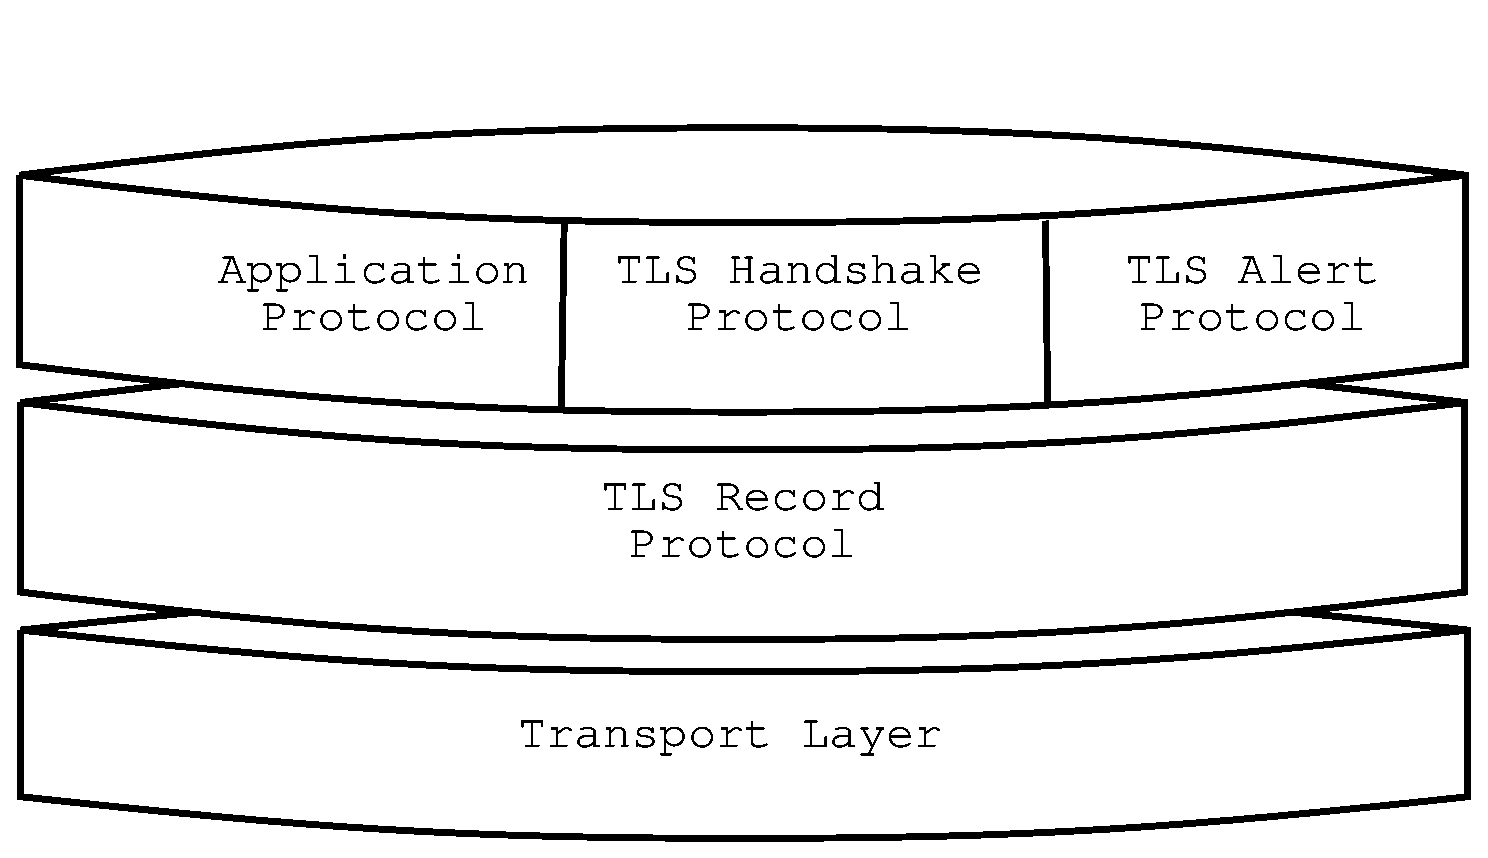
\includegraphics{layers}
\label{fig:layers}

\end{figure}


\addvspace{1.5cm}



\section{Transport Layer}
\par
\gnutls can be used above any transport layer. To do this you will only 
need to set up the 
\hyperref{gnutls\_global\_set\_push\_func()}{gnutls\_global\_set\_push\_func() (see Section }{
for more information)}{gnutls_global_set_push_func} and
\hyperref{gnutls\_global\_set\_pull\_func()}{gnutls\_global\_set\_pull\_func() (see Section }{
for more information)}{gnutls_global_set_pull_func}
functions. These functions will then be used by gnutls in order to send and receive data.
The functions specified should return -1 on error and probably set errno appropriately.
\gnutls supports EINTR and EAGAIN errno values (This means that appropriate
values will be returned to the caller of the gnutls function).
\par
By default (if the above functions are not called), gnutls will use
the berkeley sockets functions recv() and send(). In this case
gnutls will use some hacks in order for select() to work, thus
making easy to add \emph{TLS} support to existing servers.




\section{The TLS record protocol\index{TLS protocols!Record}}

The Record protocol is the secure communications provider. It's purpose
is to encrypt, authenticate and --optionally-- compress packets.
The following functions are available:
\par
\begin{itemize}
\item \printfunc{gnutls_record_send}{gnutls\_record\_send}:
to send a record packet (with application data).
\item \printfunc{gnutls_record_recv}{gnutls\_record\_recv}:
to receive a record packet (with application data).
\end{itemize}

As you may have already noticed, the functions which access the Record protocol,
are quite limited, given the importance of this protocol in \tls{}.
This is because the Record protocol's parameters are all set by
the Handshake protocol.
\par
The Record protocol initially starts with NULL parameters, which means
no encryption, and no MAC is used. Encryption and authentication begin
just after the handshake protocol has finished.

\section{Symmetric encryption algorithms}
\par
Confidentiality is provided by using block encryption algorithms like {\bf 3DES}, 
{\bf AES\footnote{AES or Advanced Encryption Standard is actually the RIJNDAEL algorithm. This is the
algorithm that will replace DES.}}, or
stream algorithms like {\bf ARCFOUR\_128\footnote{ARCFOUR\_128 is a compatible
algorithm with RSA's RC4 algorithm, which is considered to be a trade secret.}} See \hyperref{fig:ciphers}{figure }{}{fig:ciphers} for a complete list. 
Ciphers are encryption algorithms that use a single (secret) key
to encrypt and decrypt data. Block algorithms in TLS also provide protection
against statistical analysis of the data. \gnutls{} makes use of this property
thus, if you're operating in \tlsI{} mode, a random number of blocks will be
appended to the data. This will prevent eavesdroppers from guessing the 
actual data size.

\begin{figure}[hbtp]
\begin{tabular}{|l|p{9cm}|}

\hline
3DES\_CBC & 3DES\_CBC is the DES block cipher algorithm used with triple
encryption (EDE). Has 64 bits block size and is used in CBC mode.
\\
\hline
ARCFOUR\_128 & ARCFOUR is a fast stream cipher.
\\
\hline
ARCFOUR\_40 & This is the ARCFOUR cipher that is fed with a 40 bit key,
which is considered weak.
\\
\hline
AES\_CBC & AES or RIJNDAEL is the block cipher algorithm that replaces 
the old DES algorithm. Has
128 bits block size and is used in CBC mode. This is not officially
supported in TLS.
\\
\hline
TWOFISH\_CBC & TWOFISH is a block cipher algorithm by Counterpane. Has
128 bits block size and is used in CBC mode. This algorithm is not
part of TLS. It is a \gnutls{} extension.
\\
\hline
\end{tabular}
\caption{Supported cipher algorithms}
\label{fig:ciphers}
\end{figure}



\addvspace{1.5cm}

\begin{figure}[hbtp]
\begin{tabular}{|l|p{9cm}|}

\hline
MAC\_MD5 & MD5 is a hash algorithm by Ron Rivest. Outputs 128 bits of data.
\\
\hline
MAC\_SHA & SHA is a hash algorithm by NSA. Outputs 160 bits of data.
\\
\hline
\end{tabular}
\caption{Supported MAC algorithms}
\label{fig:mac}
\end{figure}



\subsection*{Compression algorithms used in the record layer}
\index{Compression algorithms}
The TLS' record layer also supports compression. The algorithms
implemented in \gnutls{} can be found in figure \ref{fig:compression}.
All the algorithms except for DEFLATE which is referenced in \cite{TLSCOMP}, should be 
considered as \gnutls' extensions\footnote{You should use \printfunc{gnutls_handshake_set_private_extensions}{gnutls\_handshake\_set\_private\_extensions}
to enable private extensions.}, and
should be advertised only when the peer is known to have a compliant client,
to avoid interoperability problems.
\par
The included algorithms perform really good when text, or other
compressable data are to be transfered, but offer nothing on already 
compressed data, such as compressed images, zipped archives etc.
These compression algorithms, may be useful in high bandwidth TLS tunnels,
and in cases where network usage has to be minimized. As a drawback, 
compression increases latency.

\par
The record layer compression in \gnutls{} is implemented based on
the paper \cite{TLSCOMP}.

\begin{figure}[hbtp]
\begin{tabular}{|l|p{9cm}|}

\hline
DEFLATE & Zlib compression, using the deflate algorithm.
\\
\hline
LZO & LZO is a very fast compression algorithm. This algorithm is only
available if the \gnutlse{} library has been initialized.
\\
\hline
\end{tabular}
\caption{Supported compression algorithms}
\label{fig:compression}
\end{figure}




\subsection*{Weaknesses and countermeasures}
\index{TLS protocols!Record}

Some weaknesses that may affect the security of the Record layer have been
found in \tlsI{} protocol. These weaknesses can be exploited by active attackers,
and exploit the facts that
\begin{enumerate}
\item \tls{} has separate alerts for ``decryption\_failed'' and ``bad\_record\_mac''
\item the decryption failure reason can be detected by timing the response time
\item the IV for CBC encrypted packets is the last block of the previous encrypted packet
\end{enumerate}

Those weaknesses were solved in \tlsII{} which is implemented in
\gnutls{}. For a detailed discussion see the archives of the TLS Working Group mailing list
and the paper \cite{CBCATT}.





\section{The TLS alert protocol}

The Alert protocol is there to allow signals to be sent between peers.
These signals are mostly used to inform the peer about the cause of
a protocol failure. Some of these signals are used internally by the
protocol and the application protocol does not have to cope with them
(see \emph{GNUTLS\_A\_CLOSE\_NOTIFY}), and others refer to the
application protocol solely (see \emph{GNUTLS\_A\_USER\_CANCELLED}).
An alert signal includes a level indication which may be either
fatal or warning. Fatal alerts always terminate the current connection,
and prevent future renegotiations using the current session ID.

\par The alert messages are protected by the record protocol, thus
the information that it's included does not leak. You must take
extreme care for the alert information not to leak, to a possible attacker
(via public logfiles etc).

\par
\begin{itemize}
\item \printfunc{gnutls_alert_send}{gnutls\_alert\_send()}:
to send an alert signal.
\item \printfunc{gnutls_alert_send_appropriate}{gnutls\_alert\_send\_appropriate()}:
to send an alert signal that depends on a given gnutls error number.
\item \printfunc{gnutls_alert_get}{gnutls\_alert\_get()}:
returns the last received alert.
\item \printfunc{gnutls_alert_get_name}{gnutls\_alert\_get\_name()}:
returns the name (in a character array) of the given alert.
\end{itemize}



\section{The TLS handshake protocol\index{TLS protocols!Handshake}}
\label{handshake}

The Handshake protocol is responsible for the ciphersuite negotiation,
the initial key exchange, and the authentication of the two peers.
This is fully controlled by the application layer, thus your program
has to set up the required parameters. Available functions to control
the handshake protocol include:

\begin{itemize}
\item \printfunc{gnutls_cipher_set_priority}{gnutls\_cipher\_set\_priority}:
to set the priority of bulk cipher algorithms.
\item \printfunc{gnutls_mac_set_priority}{gnutls\_mac\_set\_priority}:
to set the priority of MAC algorithms.
\item \printfunc{gnutls_kx_set_priority}{gnutls\_kx\_set\_priority}:
to set the priority of key exchange algorithms.
\item \printfunc{gnutls_compression_set_priority}{gnutls\_compression\_set\_priority}:
to set the priority of compression methods.
\item \printfunc{gnutls_certificate_type_set_priority}{gnutls\_certificate\_type\_set\_priority}:
to set the priority of certificate types (ie. OpenPGP, X.509).
\item \printfunc{gnutls_protocol_set_priority}{gnutls\_protocol\_set\_priority}:
to set the priority of protocol versions (ie. \sslIII{}, \tlsI).
\item \printfunc{gnutls_set_default_priority}{gnutls\_set\_default\_priority}:
to set some defaults in the current session. That way you don't have to call each
priority function, independently, but you have to live with the defaults.
\item \printfunc{gnutls_credentials_set}{gnutls\_credentials\_set}: to set the
appropriate credentials structures.
\item \printfunc{gnutls_certificate_server_set_request}
{gnutls\_certificate\_server\_set\_request}: to set
whether client certificate is required or not.
\item \printfunc{gnutls_handshake}{gnutls\_handshake}: to initiate the
handshake.
\end{itemize}

\subsection*{TLS cipher suites}
\par 
The Handshake Protocol of \tlsI{} negotiates cipher suites 
of the form \\
{\bf TLS\_DHE\_RSA\_WITH\_3DES\_CBC\_SHA}.
The usual cipher suites contain these parameters:
\begin{itemize}
\item The key exchange algorithm ---DHE\_RSA in the example.
\item The Symmetric encryption algorithm and mode ---3DES\_CBC in this
example.
\item The MAC\footnote{MAC stands for Message Authentication Code. It can
be described as a keyed hash algorithm. See RFC2104.} algorithm used for authentication.
MAC\_SHA is used in the above example.
\end{itemize}

The cipher suite negotiated in the handshake protocol will affect
the Record Protocol, by enabling encryption and data authentication.
Note that you should not over rely on \tls{} to negotiate the strongest 
available cipher suite. Do not enable ciphers and algorithms that you consider weak.
\par
The priority functions, dicussed above, allow the application layer to enable
and set priorities on the individual ciphers. It may imply that all combinations of ciphersuites
are allowed, but this is not true. For several reasons, not discussed here, some combinations 
were not defined in the \tls{} protocol. The supported ciphersuites are shown
in appendix \ref{ap:ciphersuites} on page \pageref{ap:ciphersuites}.

\addvspace{1.5cm}


\subsection*{Client authentication}
In the case of ciphersuites that use certificate authentication, the
authentication\index{Certificate authentication!Client} of the client is
optional in \tls{}. A server may request a certificate from the client -- using the
\printfunc{gnutls_certificate_server_set_request}{gnutls\_certificate\_server\_set\_request}
function. If a certificate is to be requested from the client during the handshake,
the server will send a certificate request message that contains
a list of acceptable certificate signers. The client may then send a certificate, signed
by one of the server's acceptable signers. In \gnutls{} the server's acceptable
signers list is constructed using the trusted CA certificates in the
credentials structure.

\subsection*{Resuming Sessions\index{Resuming sessions}}
\label{resume}
\par
The 
\printfunc{gnutls_handshake}{gnutls\_handshake}
 function, is expensive since a lot of calculations are performed. In order to support many fast connections to
the same server a client may use session resuming. {\bf Session resuming} is a
feature of the {\bf TLS} protocol which allows a client to connect to a server,
after a successful handshake, without the expensive calculations. This is
achieved by using the previously
established keys. \gnutls{} supports this feature, and the
example \hyperref{resume client}{resume client (see section }{)}{resume-example} illustrates a typical use of it.
\par
Keep in mind that sessions are expired after some time, for security reasons, thus
it may be normal for a server not to resume a session even if you requested that.
Also note that you must enable, using the priority functions, at least the
algorithms used in the last session.

\subsection*{Resuming internals}
The resuming capability, mostly in the server side, is one of the problems of a thread-safe TLS
implementations. The problem is that all threads must share information in
order to be able to resume sessions. The gnutls approach is, in case of a
client, to leave all the burden of resuming to the client. Ie. copy and keep the
necessary parameters. See the functions:
\begin{itemize}
\item \printfunc{gnutls_session_get_data}{gnutls\_session\_get\_data}
\item \printfunc{gnutls_session_get_id}{gnutls\_session\_get\_id}
\item \printfunc{gnutls_session_set_data}{gnutls\_session\_set\_data}
\end{itemize}

\par
The server side is different. A server has to specify some callback functions
which store, retrieve and delete session data. These can be registered with:
\begin{itemize}
\item \printfunc{gnutls_db_set_remove_function}{gnutls\_db\_set\_remove\_function}
\item \printfunc{gnutls_db_set_store_function}{gnutls\_db\_set\_store\_function}
\item \printfunc{gnutls_db_set_retrieve_function}{gnutls\_db\_set\_retrieve\_function}
\item \printfunc{gnutls_db_set_ptr}{gnutls\_db\_set\_ptr}
\end{itemize}

\par
It might also be useful to be able to check for expired sessions in order to remove 
them, and save space. The function
\printfunc{gnutls_db_check_entry}{gnutls\_db\_check\_entry} is provided for that
reason.




\chapter{Authentication methods}
\par
The following authentication schemas are supported in \gnutls:
\begin{enumerate}
 \item Certificate authentication
 \item Anonymous authentication
 \item SRP authentication
\end{enumerate}

% x.509 section
\section{Authentication using X.509\index{X.509 certificates} certificates}

This authentication method is part of the certificate authentication
method in \gnutls{}.
The X.509 protocols rely on a hierarchical trust model. In this trust model
Certification Authorities (CAs) are used to certify entities.
Usually more than one certification authorities exist, and certification
authorities may certify other authorities to issue certificates as well,
following a hierachical model. 
One needs to trust one or more CAs for his secure
communications. In that case only the certificates issued by the trusted
authorities are acceptable. 
\par
X.509 certificates contain the public parameters, 
of a public key algorithm, and the authority's signature, which proves the
authenticity of the parameters.
\par
The key exchange methods shown in \hyperref{figure}{figure }{}{fig:cert} are
available in X.509 authentication. 

\par The use of X.509 certificates requires some functions which will 
assist in parsing them. \gnutls{} includes functions which extract 
parameters from given X.509 certificates. Some of them are:
\begin{itemize}
\item \printfunc{gnutls_x509_extract_certificate_dn}{gnutls\_x509\_extract\_certificate\_dn}
\item \printfunc{gnutls_x509_extract_certificate_serial}{gnutls\_x509\_extract\_certificate\_serial}
\item \printfunc{gnutls_x509_extract_certificate_subject_alt_name}{gnutls\_x509\_extract\_certificate\_subject\_alt\_name}
\end{itemize}

Given the complexity of the X.509 protocols we do not expect these limited 
functions to cover every need. Thus a function which exports X.509 certificates
to an XML form is provided. See 
\printfunc{gnutls_x509_get_certificate_xml}{gnutls\_x509\_get\_certificate\_xml}.

\par
Verifying certificate\index{Verifying certificate paths} paths is also important in X.509 authentication.
For this purpose you can use the
\printfunc{gnutls_x509_verify_certificate}{gnutls\_x509\_verify\_certificate}
function. A more generic one is also provided and can be used with all
of the certificate authentication methods, but is limited to a session. See the
\printfunc{gnutls_certificate_verify_peers}{gnutls\_certificate\_verify\_peers}
function.

\par
Note that \gnutls{} is not a generic purpose X.509 toolkit\footnote{Aegypten is such a toolkit. See 
\htmladdnormallink{http://www.gnupg.org/aegypten/}{http://www.gnupg.org/aegypten/}}. 
\gnutls{} only includes the required,
in order to use the TLS ciphersuites which require X.509 certificates.



\begin{figure}[hbtp]
\begin{tabular}{|l|p{9cm}|}
\hline
RSA & The RSA algorithm is used to encrypt a key and send it to the peer.
The certificate must allow the key to be used for encryption.
\\
\hline
RSA\_EXPORT & The RSA algorithm is used to encrypt a key and send it to the peer.
In the EXPORT algorithm, the server signs temporary RSA parameters of 512
bits -- which are considered weak -- and sends them to the client.
\\
\hline
DHE\_RSA & The RSA algorithm is used to sign Ephemeral Diffie Hellman
parameters which are sent to the peer. The key in the certificate must allow
the key to be used for signing. Note that key exchange algorithms which use
Ephemeral Diffie Hellman parameters, offer perfect forward secrecy.
\\
\hline
DHE\_DSS & The DSS\footnote{DSS stands for Digital Signature Standard} algorithm is used to sign Ephemeral Diffie Hellman
parameters which are sent to the peer. 
\\
\hline
\end{tabular}

\caption{Key exchange algorithms for OpenPGP and X.509 certificates.}
\label{fig:cert}

\end{figure}


% openpgp section

\section{Authentication using OpenPGP\index{OpenPGP keys} keys}
\label{sec:pgp}

This authentication method is part of the certificate authentication
method in \gnutls{}. All the key exchange methods shown in \hyperref{figure}{figure }{}{fig:cert} are
available in OpenPGP authentication. The \gnutls{}'s implementation is based on the
\cite{TLSPGP} proposal.

See \ref{pgp:trust} on page \pageref{pgp:trust} for more information 
about the OpenPGP trust model.




\section{Anonymous authentication\index{Anonymous authentication}}
The anonymous key exchange perform encryption but there is no indication of 
the identity of the peer. This kind of authentication is vulnerable to a
man in the middle attack, 
but this protocol can be used even if there is no prior communication or common trusted
parties with the peer. Unless really required, do not use anonymous authentication.
Available key exchange methods are shown in \hyperref{figure}{figure }{}{fig:anon}.

\begin{figure}[hbtp]
\begin{tabular}{|l|p{9cm}|}

\hline
ANON\_DH & This algorithm exchanges Diffie Hellman parameters. 
\\
\hline
\end{tabular}

\caption{Supported anonymous key exchange algorithms}
\label{fig:anon}

\end{figure}

\section{Authentication using SRP\index{SRP authentication}}
Authentication using the SRP\footnote{SRP stands for Secure Password Protocol and 
is described in RFC2945. The SRP key exchange is not a part of the \tlsI{} protocol}
is actually password authentication, since the two peers are identified by the knowledge of a password. 
This protocol also offers protection against off-line attacks, such as password 
file stealing. 
This is achieved since SRP does not use the plain password to perform authentication, but something called a 
verifier. The verifier is $g^{x}mod(n)$ and $x$ is a value calculated
from the username and the password. 
\par SRP is normaly used with a SHA based hash function, to calculate
the value of $x$. 
\par The advantage of SRP authentication, over other proposed secure password 
authentication schemas, is that SRP does not require the server to hold
the user's password. This kind of protection is similar to the one used traditionaly
in the \emph{UNIX} ``passwd'' file, where the contents of this file did not cause
harm to the system security if they were revealed.
\par
Available key exchange methods are shown in \hyperref{figure}{figure }{}{fig:srp}.

\begin{figure}[hbtp]
\begin{tabular}{|l|p{9cm}|}

\hline
SRP & Authentication using the SRP protocol. 
\\
\hline
\end{tabular}

\caption{Supported SRP key exchange algorithms}
\label{fig:srp}

\end{figure}

\gnutls{} includes a program to manipulate the required for SRP
authentication. See \ref{srpcrypt} on page \pageref{srpcrypt} for
more information.


\section{Error Handling}
\par
In \gnutls most functions return an integer type as a result.
In almost all cases a zero or a positive number means success, and
a negative number indicates failure, or a situation that some
action has to be taken. Thus negative error codes may be fatal
or not. 
\par 
Fatal errors terminate the connection immediately and
further sends ard receives will be disallowed. An example of
a fatal error code is GNUTLS\_E\_MAC\_FAILED. Non-fatal errors
may warn about something (ie a warning alert was received), or
indicate the some action has to be taken. This is the case with
the error code GNUTLS\_E\_REHANDSHAKE returned by 
\hyperref{gnutls\_record\_recv()}{gnutls\_record\_recv() (see Section }{)}{gnutls_record_recv}.
This error code indicates that the server requests a rehandshake. The client
may ignore this request, or may reply with an alert.
You can test if an error code is a fatal one by using the
\hyperref{gnutls\_error\_is\_fatal()}{gnutls\_error\_is\_fatal() (see Section }{)}{gnutls_error_is_fatal}.
\par
If any non fatal errors, that require reaction, are to be returned by a
function, these error codes will be documented
in the function's reference.



\section{Memory handling}

\gnutls{} internally handles heap allocated objects differently, depending
on the sensitivity of the data they contain. However for performance
reasons, the default memory functions do not overwrite sensitive data from
memory, nor protect such objects from being written to the swap. 
In order to change the default behavior the
\printfunc{gnutls_global_set_mem_functions}{gnutls\_global\_set\_mem\_functions}
function is available which can be used to set other memory 
handlers than the defaults. 
\par
The \emph{libgcrypt} library on which \gnutls{} depends, has such secure
memory allocation functions available. These should be used in cases
where even the system's swap memory is not considered secure. See
the documentation of \emph{libgcrypt} for more information.




\chapter{How to use \gnutls{}\index{Example programs} in applications}

%\section{Preparation\footnote{This section is heavily based on the `libksba' documentation}}
\section{Preparation}

To use \gnutls{}, you have to perform some changes to your sources and
your build system. The necessary changes are explained in the following
subsections.

\subsection*{Headers}

All the data types and functions of the \gnutls{} library are defined in
the header file `gnutls/gnutls.h'. This must be included in all programs that
make use of the \gnutls{} library.
\par
The extra functionality of the \gnutlse{} library is available by
including the header file `gnutls/extra.h' in your programs.

\subsection*{Version check}
It is often desirable to check that the version of `gnutls' used is indeed
one which fits all requirements.  Even with binary compatibility new
features may have been introduced but due to problem with the dynamic
linker an old version is actually used.  So you may want to check that
the version is okay right after program startup.
See the function \printfunc{gnutls_check_version}{gnutls\_check\_version}


\subsection*{Building the source}

If you want to compile a source file including the `gnutls/gnutls.h' header
file, you must make sure that the compiler can find it in the
directory hierarchy.  This is accomplished by adding the path to the
directory in which the header file is located to the compilers include
file search path (via the -I option).

However, the path to the include file is determined at the time the
source is configured.  To solve this problem, \gnutls{} ships with two small
helper programs \command{libgnutls-config} and \command{libgnutls-extra-config}
that knows about the path to the
include file and other configuration options.  The options that need
to be added to the compiler invocation at compile time are output by
the \option{--cflags} option to \option{libgnutls-config}.  The following
example shows how it can be used at the command line:

\begin{verbatim}
gcc -c foo.c `libgnutls-config --cflags`
\end{verbatim}

Adding the output of \command{libgnutls-config --cflags} to the compilers
command line will ensure that the compiler can find the \gnutls{} header
file.

A similar problem occurs when linking the program with the library.
Again, the compiler has to find the library files.  For this to work,
the path to the library files has to be added to the library search
path (via the -L option).  For this, the option
\option{--libs} to \command{libgnutls-config} can be used.  For
convenience, this option also outputs all other options that are
required to link the program with the \gnutls{} libararies.
The example shows how to link `foo.o'
with the \gnutls{} libraries to a program \emph{foo}.

\begin{verbatim}
gcc -o foo foo.o `libgnutls-config --libs`
\end{verbatim}

Of course you can also combine both examples to a single command by
specifying both options to `libgnutls-config':

\begin{verbatim}
gcc -o foo foo.c `libgnutls-config --cflags --libs`
\end{verbatim}



\label{examples}
\section{Client examples}
This section contains examples of \tls{} and \ssl{} clients, using \gnutls{}. 
Note that these examples contain little or no error checking.

\subsection{Simple client example with X.509 certificate support}
Let's assume now that we want to create a TCP client which communicates
with servers that use X.509 or OpenPGP certificate authentication. The following client
is a very simple \tls{} client, it does not support session resuming, not
even certificate verification. The TCP functions defined in this example
are used in most of the other examples below, without redefining them.
\begin{verbatim}

#include <stdio.h>
#include <stdlib.h>
#include <sys/types.h>
#include <sys/socket.h>
#include <netinet/in.h>
#include <arpa/inet.h>
#include <unistd.h>
#include <gnutls/gnutls.h>

/* A very basic TLS client.
 */

#define MAX_BUF 1024
#define CRLFILE "crl.pem"
#define CAFILE "ca.pem"
#define SA struct sockaddr
#define MSG "GET / HTTP/1.0\r\n\r\n"

int main()
{
   const char *PORT = "443";
   const char *SERVER = "127.0.0.1";
   int err, ret;
   int sd, ii;
   struct sockaddr_in sa;
   gnutls_session session;
   char buffer[MAX_BUF + 1];
   gnutls_certificate_client_credentials xcred;
   const int protocol_priority[] = { GNUTLS_TLS1, GNUTLS_SSL3, 0 };
   const int kx_priority[] = { GNUTLS_KX_RSA, 0 };
   const int cipher_priority[] = { GNUTLS_CIPHER_3DES_CBC, GNUTLS_CIPHER_ARCFOUR_128, 0};
   const int comp_priority[] = { GNUTLS_COMP_NULL, 0 };
   const int mac_priority[] = { GNUTLS_MAC_SHA, GNUTLS_MAC_MD5, 0 };


   gnutls_global_init();

   /* X509 stuff */
   gnutls_certificate_allocate_credentials(&xcred);

   /* set's the trusted cas file
    */
   gnutls_certificate_set_x509_trust_file(xcred, CAFILE, GNUTLS_X509_FMT_PEM);

   /* connects to server 
    */
   sd = socket(AF_INET, SOCK_STREAM, 0);

   memset(&sa, '\0', sizeof(sa));
   sa.sin_family = AF_INET;
   sa.sin_port = htons(atoi(PORT));
   inet_pton(AF_INET, SERVER, &sa.sin_addr);

   err = connect(sd, (SA *) & sa, sizeof(sa));
   if (err < 0) {
      fprintf(stderr, "Connect error\n");
      exit(1);
   }
   /* Initialize TLS session 
    */
   gnutls_init(&session, GNUTLS_CLIENT);

   /* allow both SSL3 and TLS1
    */
   gnutls_protocol_set_priority(session, protocol_priority);

   /* allow only ARCFOUR and 3DES ciphers
    * (3DES has the highest priority)
    */
   gnutls_cipher_set_priority(session, cipher_priority);

   /* only allow null compression
    */
   gnutls_compression_set_priority(session, comp_priority);

   /* use GNUTLS_KX_RSA
    */
   gnutls_kx_set_priority(session, kx_priority);

   /* allow the usage of both SHA and MD5
    */
   gnutls_mac_set_priority(session, mac_priority);


   /* put the x509 credentials to the current session
    */
   gnutls_credentials_set(session, GNUTLS_CRD_CERTIFICATE, xcred);


   gnutls_transport_set_ptr( session, sd);
   /* Perform the TLS handshake
    */
   ret = gnutls_handshake( session);

   if (ret < 0) {
      fprintf(stderr, "*** Handshake failed\n");
      gnutls_perror(ret);
      goto end;
   } else {
      printf("- Handshake was completed\n");
   }

   gnutls_record_send( session, MSG, strlen(MSG));

   ret = gnutls_record_recv( session, buffer, MAX_BUF);
   if (ret == 0) {
      printf("- Peer has closed the TLS connection\n");
      goto end;
   } else if (ret < 0) {
      fprintf(stderr, "*** Received corrupted data(%d) - server has terminated the connection abnormally\n",
              ret);
      goto end;
   } else if (ret > 0) {
      printf("- Received %d bytes: ", ret);
      for (ii = 0; ii < ret; ii++) {
         fputc(buffer[ii], stdout);
      }
      fputs("\n", stdout);
   }
   gnutls_bye( session, GNUTLS_SHUT_RDWR);

 end:

   shutdown(sd, SHUT_RDWR);     /* no more receptions */
   close(sd);

   gnutls_deinit(session);

   gnutls_certificate_free_credentials(xcred);

   gnutls_global_deinit();

   return 0;
}

\end{verbatim}


\subsection{Obtaining session information}
Most of the times it is desirable to know the security properties of
the current established session. This includes the underlying ciphers and
the protocols involved. That is the purpose of the following function.
Note that this function will print meaningful values only if
called after a successful \printfunc{gnutls_handshake}{gnutls\_handshake}

\begin{verbatim}

#include <stdio.h>
#include <stdlib.h>
#include <gnutls/gnutls.h>
#include <gnutls/x509.h>

extern void print_x509_certificate_info(gnutls_session);

/* This function will print some details of the
 * given session.
 */
int print_info(gnutls_session session)
{
   const char *tmp;
   gnutls_credentials_type cred;
   gnutls_kx_algorithm kx;

   /* print the key exchange's algorithm name
    */
   kx = gnutls_kx_get(session);
   tmp = gnutls_kx_get_name(kx);
   printf("- Key Exchange: %s\n", tmp);

   /* Check the authentication type used and switch
    * to the appropriate.
    */
   cred = gnutls_auth_get_type(session);
   switch (cred) {
   case GNUTLS_CRD_ANON:       /* anonymous authentication */

      printf("- Anonymous DH using prime of %d bits\n",
             gnutls_dh_get_prime_bits(session));
      break;

   case GNUTLS_CRD_CERTIFICATE:        /* certificate authentication */
      
      /* Check if we have been using ephemeral Diffie Hellman.
       */
      if (kx == GNUTLS_KX_DHE_RSA || kx == GNUTLS_KX_DHE_DSS) {
         printf("\n- Ephemeral DH using prime of %d bits\n",
                gnutls_dh_get_prime_bits(session));
      }

      /* if the certificate list is available, then
       * print some information about it.
       */
      print_x509_certificate_info(session);

   } /* switch */

   /* print the protocol's name (ie TLS 1.0) 
    */
   tmp = gnutls_protocol_get_name(gnutls_protocol_get_version(session));
   printf("- Protocol: %s\n", tmp);

   /* print the certificate type of the peer.
    * ie X.509
    */
   tmp = gnutls_certificate_type_get_name(
      gnutls_certificate_type_get(session));

   printf("- Certificate Type: %s\n", tmp);

   /* print the compression algorithm (if any)
    */
   tmp = gnutls_compression_get_name( gnutls_compression_get(session));
   printf("- Compression: %s\n", tmp);

   /* print the name of the cipher used.
    * ie 3DES.
    */
   tmp = gnutls_cipher_get_name(gnutls_cipher_get(session));
   printf("- Cipher: %s\n", tmp);

   /* Print the MAC algorithms name.
    * ie SHA1
    */
   tmp = gnutls_mac_get_name(gnutls_mac_get(session));
   printf("- MAC: %s\n", tmp);

   return 0;
}

\end{verbatim}


\subsection{Verifying peer's certificate}
A \tls{} session is not secure just after the handshake procedure has finished.
It must be considered secure, only after the peer's certificate and identity have been
verified. That is, you have to verify the signature in peer's 
certificate, the hostname in the certificate, and expiration dates.
Just after this step you should treat the connection as being a secure one.
The following function is an example on how to verify the peer's certificate chain.
This is an advanced case. Things in a TLS session may be simplified by using
\printfunc{gnutls_certificate_verify_peers2}{gnutls\_certificate\_verify\_peers2}.

\index{Verifying certificate chains}
\label{ex:verify-chain}

\begin{verbatim}

#include <stdio.h>
#include <gnutls/gnutls.h>
#include <gnutls/x509.h>

/* All the available CRLs
 */
extern gnutls_x509_crl* crl_list;
extern int crl_list_size;

/* All the available trusted CAs
 */
extern gnutls_x509_crt* ca_list;
extern int ca_list_size;

static void verify_cert2(gnutls_x509_crt crt,
	gnutls_x509_crt issuer, gnutls_x509_crl * crl_list, int crl_list_size);
static void verify_last_cert(gnutls_x509_crt crt,
   gnutls_x509_crt *ca_list, int ca_list_size,
   gnutls_x509_crl * crl_list, int crl_list_size);


/* This function will try to verify the peer's certificate chain, and
 * also check if the hostname matches, and the activation, expiration dates.
 */
void verify_certificate_chain( gnutls_session session, const char* hostname,
   const gnutls_datum* cert_chain, int cert_chain_length)
{
   int i, ret;
   gnutls_x509_crt cert[cert_chain_length];

   /* Import all the certificates in the chain to
    * native certificate format.
    */
   for (i=0;i<cert_chain_length;i++) {
      gnutls_x509_crt_init(&cert[i]);
      gnutls_x509_crt_import( cert[i], &cert_chain[i], GNUTLS_X509_FMT_DER);
   }

   /* Now verify the certificates against their issuers
    * in the chain.
    */   
   for (i=1;i<cert_chain_length;i++) {
      verify_cert2( cert[i-1], cert[i], crl_list, crl_list_size);
   }

   /* Here we must verify the last certificate in the chain against
    * our trusted CA list.
    */
   verify_last_cert( cert[cert_chain_length-1], 
      ca_list, ca_list_size, crl_list, crl_list_size);

   /* Check if the name in the first certificate matches our destination!
    */
   if ( !gnutls_x509_crt_check_hostname( cert[0], hostname)) {
      printf("The certificate's owner does not match hostname '%s'\n", hostname);
   }

   for (i=0;i<cert_chain_length;i++)
      gnutls_x509_crt_deinit( cert[i]);

   return;
}


/* Verifies a certificate against an other certificate
 * which is supposed to be it's issuer. Also checks the
 * crl_list if the certificate is revoked.
 */
static void verify_cert2(gnutls_x509_crt crt,
   gnutls_x509_crt issuer, gnutls_x509_crl * crl_list, int crl_list_size)
{ 
   unsigned int output;
   int ret;
   time_t now = time(0);
   size_t name_size;
   char name[64];

   /* Print information about the certificates to
    * be checked.
    */
   name_size = sizeof(name);
   gnutls_x509_crt_get_dn( crt, name, &name_size);

   fprintf(stderr, "\nCertificate: %s\n", name);

   name_size = sizeof(name);
   gnutls_x509_crt_get_issuer_dn(crt, name, &name_size);

   fprintf(stderr, "Issued by: %s\n", name);

   /* Get the DN of the issuer cert.
    */
   name_size = sizeof(name);
   gnutls_x509_crt_get_dn(issuer, name, &name_size);

   fprintf(stderr, "Checking against: %s\n", name);

   /* Do the actual verification.
    */
   gnutls_x509_crt_verify(crt, &issuer, 1, 0, &output);

   if (output & GNUTLS_CERT_INVALID) {
      fprintf(stderr, "Not trusted");

      if (output & GNUTLS_CERT_SIGNER_NOT_CA)
         fprintf(stderr, ": Issuer is not a CA\n");
      else
         fprintf(stderr, "\n");
   } else
      fprintf(stderr, "Trusted\n");


    /* Now check the expiration dates.
     */
    if (gnutls_x509_crt_get_activation_time(crt) > now)
	fprintf(stderr, "Not yet activated\n");

    if (gnutls_x509_crt_get_expiration_time(crt) < now)
	fprintf(stderr, "Expired\n");

    /* Check if the certificate is revoked.
     */
    ret = gnutls_x509_crt_check_revocation(crt, crl_list, crl_list_size);
    if (ret == 1) {		/* revoked */
	fprintf(stderr, "Revoked\n");
    }
}


/* Verifies a certificate against the trusted CA list.
 * Also checks the crl_list if the certificate is revoked.
 */
static void verify_last_cert(gnutls_x509_crt crt,
   gnutls_x509_crt *ca_list, int ca_list_size,
   gnutls_x509_crl * crl_list, int crl_list_size)
{ 
   unsigned int output;
   int ret;
   time_t now = time(0);
   size_t name_size;
   char name[64];

   /* Print information about the certificates to
    * be checked.
    */
   name_size = sizeof(name);
   gnutls_x509_crt_get_dn( crt, name, &name_size);

   fprintf(stderr, "\nCertificate: %s\n", name);

   name_size = sizeof(name);
   gnutls_x509_crt_get_issuer_dn(crt, name, &name_size);

   fprintf(stderr, "Issued by: %s\n", name);

   /* Do the actual verification.
    */
   gnutls_x509_crt_verify(crt, ca_list, ca_list_size, 0, &output);

   if (output & GNUTLS_CERT_INVALID) {
      fprintf(stderr, "Not trusted");

      if (output & GNUTLS_CERT_SIGNER_NOT_CA)
         fprintf(stderr, ": Issuer is not a CA\n");
      else
         fprintf(stderr, "\n");
   } else
      fprintf(stderr, "Trusted\n");


    /* Now check the expiration dates.
     */
    if (gnutls_x509_crt_get_activation_time(crt) > now)
	fprintf(stderr, "Not yet activated\n");

    if (gnutls_x509_crt_get_expiration_time(crt) < now)
	fprintf(stderr, "Expired\n");

    /* Check if the certificate is revoked.
     */
    ret = gnutls_x509_crt_check_revocation(crt, crl_list, crl_list_size);
    if (ret == 1) {		/* revoked */
	fprintf(stderr, "Revoked\n");
    }
}

\end{verbatim}


\subsection{Using a callback to select the certificate to use}
There are cases where a client holds several certificate and key pairs,
and may not want to load all of them in the credentials structure.
The following example demonstrates the use of the certificate selection callback.
\par

\begin{verbatim}

#include <stdio.h>
#include <stdlib.h>
#include <string.h>
#include <sys/types.h>
#include <sys/socket.h>
#include <netinet/in.h>
#include <arpa/inet.h>
#include <unistd.h>
#include <sys/mman.h>
#include <sys/stat.h>
#include <gnutls/gnutls.h>
#include <gnutls/x509.h>

/* A TLS client that loads the certificate and key.
 */

#define MAX_BUF 1024
#define SA struct sockaddr
#define MSG "GET / HTTP/1.0\r\n\r\n"

#define CERT_FILE "cert.pem"
#define KEY_FILE "key.pem"
#define CAFILE "ca.pem"

static int cert_callback(gnutls_session session,
                  const gnutls_datum* req_ca_rdn, int nreqs,
                  gnutls_retr_st * st);

gnutls_x509_crt crt;
gnutls_x509_privkey key;

/* Helper functions to load a certificate and key
 * files into memory. They use mmap for simplicity.
 */
static gnutls_datum mmap_file( const char* file)
{
int fd;
gnutls_datum mmaped_file = { NULL, 0 };
struct stat stat_st;
void* ptr;

   fd = open( file, 0);
   if (fd==-1) return mmaped_file;
   
   fstat( fd, &stat_st);
   
   if ((ptr=mmap( NULL, stat_st.st_size, PROT_READ, MAP_SHARED, fd, 0)) == MAP_FAILED)
      return mmaped_file;
   
   mmaped_file.data = ptr;
   mmaped_file.size = stat_st.st_size;
   
   return mmaped_file;
}

static void munmap_file( gnutls_datum data)
{
   munmap( data.data, data.size);
}

/* Load the certificate and the private key.
 */
static void load_keys( void)
{
int ret;
gnutls_datum data;

   data = mmap_file( CERT_FILE);
   if (data.data == NULL) {
      fprintf(stderr, "*** Error loading cert file.\n");
      exit(1);
   }
   gnutls_x509_crt_init( &crt);
   
   ret = gnutls_x509_crt_import( crt, &data, GNUTLS_X509_FMT_PEM);
   if (ret < 0) {
      fprintf(stderr, "*** Error loading key file: %s\n", gnutls_strerror(ret));
      exit(1);
   }

   munmap_file( data);

   data = mmap_file( KEY_FILE);
   if (data.data == NULL) {
      fprintf(stderr, "*** Error loading key file.\n");
      exit(1);
   }

   gnutls_x509_privkey_init( &key);
   
   ret = gnutls_x509_privkey_import( key, &data, GNUTLS_X509_FMT_PEM);
   if (ret < 0) {
      fprintf(stderr, "*** Error loading key file: %s\n", gnutls_strerror(ret));
      exit(1);
   }

   munmap_file( data);
   
}

int main()
{
   int ret, sd, ii;
   gnutls_session session;
   char buffer[MAX_BUF + 1];
   gnutls_certificate_credentials xcred;
   /* Allow connections to servers that have OpenPGP keys as well.
    */

   gnutls_global_init();

   load_keys();

   /* X509 stuff */
   gnutls_certificate_allocate_credentials(&xcred);

   /* sets the trusted cas file
    */
   gnutls_certificate_set_x509_trust_file(xcred, CAFILE, GNUTLS_X509_FMT_PEM);

   gnutls_certificate_client_set_retrieve_function( xcred, cert_callback);
   
   /* Initialize TLS session 
    */
   gnutls_init(&session, GNUTLS_CLIENT);

   /* Use default priorities */
   gnutls_set_default_priority(session);

   /* put the x509 credentials to the current session
    */
   gnutls_credentials_set(session, GNUTLS_CRD_CERTIFICATE, xcred);

   /* connect to the peer
    */
   sd = tcp_connect();

   gnutls_transport_set_ptr( session, (gnutls_transport_ptr)sd);

   /* Perform the TLS handshake
    */
   ret = gnutls_handshake( session);

   if (ret < 0) {
      fprintf(stderr, "*** Handshake failed\n");
      gnutls_perror(ret);
      goto end;
   } else {
      printf("- Handshake was completed\n");
   }

   gnutls_record_send( session, MSG, strlen(MSG));

   ret = gnutls_record_recv( session, buffer, MAX_BUF);
   if (ret == 0) {
      printf("- Peer has closed the TLS connection\n");
      goto end;
   } else if (ret < 0) {
      fprintf(stderr, "*** Error: %s\n", gnutls_strerror(ret));
      goto end;
   }

   printf("- Received %d bytes: ", ret);
   for (ii = 0; ii < ret; ii++) {
      fputc(buffer[ii], stdout);
   }
   fputs("\n", stdout);

   gnutls_bye( session, GNUTLS_SHUT_RDWR);

 end:

   tcp_close( sd);

   gnutls_deinit(session);

   gnutls_certificate_free_credentials(xcred);

   gnutls_global_deinit();

   return 0;
}



/* This callback should be associated with a session by calling
 * gnutls_certificate_client_set_retrieve_function( session, cert_callback),
 * before a handshake.
 */

static int cert_callback(gnutls_session session,
                  const gnutls_datum* req_ca_rdn, int nreqs,
                  gnutls_retr_st * st)
{
   char issuer_dn[256];
   int i, ret;
   size_t len;
   gnutls_certificate_type type;

   /* Print the server's trusted CAs
    */
   if (nreqs > 0)
      printf("- Server's trusted authorities:\n");
   else
      printf("- Server did not send us any trusted authorities names.\n");

   /* print the names (if any) */
   for (i = 0; i < nreqs; i++) {
      len = sizeof(issuer_dn);
      ret = gnutls_x509_rdn_get(&req_ca_rdn[i], issuer_dn, &len);
      if (ret >= 0) {
         printf("   [%d]: ", i);
         printf("%s\n", issuer_dn);
      }
   }

   /* Select a certificate and return it.
    */

   type = gnutls_certificate_type_get( session);
   if (type == GNUTLS_CRT_X509) {
      st->type = type;
      st->ncerts = 1;

      st->cert.x509 = &crt;
      st->key.x509 = key;

      st->deinit_all = 0;
   } else {
      return -1;
   }

   return 0;

}

\end{verbatim}



\subsection{Client with Resume capability example}
\label{resume-example}
This is a modification of the simple client example. Here we demonstrate
the use of session resumption. The client tries to connect once using
\tls{}, close the connection and then try to establish a new connection
using the previously negotiated data.
\begin{verbatim}

#include <stdio.h>
#include <stdlib.h>
#include <gnutls/gnutls.h>

/* Those functions are defined in other examples.
 */
extern void check_alert(gnutls_session session, int ret);
extern int tcp_connect( void);
extern void tcp_close( int sd);

#define MAX_BUF 1024
#define CRLFILE "crl.pem"
#define CAFILE "ca.pem"
#define SA struct sockaddr
#define MSG "GET / HTTP/1.0\r\n\r\n"

int main()
{
   int ret;
   int sd, ii, alert;
   gnutls_session session;
   char buffer[MAX_BUF + 1];
   gnutls_certificate_credentials xcred;

   /* variables used in session resuming 
    */
   int t;
   char *session_data;
   size_t session_data_size;

   gnutls_global_init();

   /* X509 stuff */
   gnutls_certificate_allocate_credentials(&xcred);

   gnutls_certificate_set_x509_trust_file(xcred, CAFILE, GNUTLS_X509_FMT_PEM);

   for (t = 0; t < 2; t++) {    /* connect 2 times to the server */

      sd = tcp_connect();

      gnutls_init(&session, GNUTLS_CLIENT);

      gnutls_set_default_priority(session);

      gnutls_credentials_set(session, GNUTLS_CRD_CERTIFICATE, xcred);

      if (t > 0) { /* if this is not the first time we connect */
         gnutls_session_set_data(session, session_data, session_data_size);
         free(session_data);
      }
      
      gnutls_transport_set_ptr( session, (gnutls_transport_ptr)sd);

      /* Perform the TLS handshake
       */
      ret = gnutls_handshake( session);

      if (ret < 0) {
         fprintf(stderr, "*** Handshake failed\n");
         gnutls_perror(ret);
         goto end;
      } else {
         printf("- Handshake was completed\n");
      }

      if (t == 0) { /* the first time we connect */
         /* get the session data size */
         gnutls_session_get_data(session, NULL, &session_data_size);
         session_data = malloc(session_data_size);

         /* put session data to the session variable */
         gnutls_session_get_data(session, session_data, &session_data_size);

      } else { /* the second time we connect */

         /* check if we actually resumed the previous session */
         if (gnutls_session_is_resumed( session) != 0) {
            printf("- Previous session was resumed\n");
         } else {
            fprintf(stderr, "*** Previous session was NOT resumed\n");
         }
      }

      /* This function was defined in a previous example
       */
      /* print_info(session); */

      gnutls_record_send( session, MSG, strlen(MSG));

      ret = gnutls_record_recv( session, buffer, MAX_BUF);
      if (ret == 0) {
         printf("- Peer has closed the TLS connection\n");
         goto end;
      } else if (ret < 0) {
         fprintf(stderr, "*** Error: %s\n", gnutls_strerror(ret));
         goto end;
      }

      printf("- Received %d bytes: ", ret);
      for (ii = 0; ii < ret; ii++) {
         fputc(buffer[ii], stdout);
      }
      fputs("\n", stdout);

      gnutls_bye( session, GNUTLS_SHUT_RDWR);

    end:

      tcp_close(sd);

      gnutls_deinit(session);

   }  /* for() */

   gnutls_certificate_free_credentials(xcred);

   gnutls_global_deinit();

   return 0;
}

\end{verbatim}


\subsection{Simple client example with SRP authentication}
The following client
is a very simple SRP \tls{} client which connects to a server 
and authenticates using a {\it username} and a {\it password}. The
server may authenticate itself using a certificate, and in that case it
has to be verified.
\begin{verbatim}

#include <stdio.h>
#include <stdlib.h>
#include <gnutls/gnutls.h>
#include <gnutls/extra.h>

/* Those functions are defined in other examples.
 */
extern void check_alert(gnutls_session session, int ret);
extern int tcp_connect( void);
void tcp_close( int sd);

#define MAX_BUF 1024
#define USERNAME "user"
#define PASSWORD "pass"
#define SA struct sockaddr
#define MSG "GET / HTTP/1.0\r\n\r\n"

const int kx_priority[] = { GNUTLS_KX_SRP, 0 };

int main()
{
   int ret;
   int sd, ii;
   gnutls_session session;
   char buffer[MAX_BUF + 1];
   gnutls_srp_client_credentials xcred;

   if (gnutls_global_init() < 0) {
      fprintf(stderr, "global state initialization error\n");
      exit(1);
   }

   /* now enable the gnutls-extra library which contains the
    * SRP stuff. */
   if (gnutls_global_init_extra() < 0) {
      fprintf(stderr, "global state initialization error\n");
      exit(1);
   }

   if (gnutls_srp_allocate_client_credentials(&xcred) < 0) {
      fprintf(stderr, "memory error\n");
      exit(1);
   }
   gnutls_srp_set_client_credentials(xcred, USERNAME, PASSWORD);

   /* connects to server 
    */
   sd = tcp_connect();

   /* Initialize TLS session 
    */
   gnutls_init(&session, GNUTLS_CLIENT);


   /* Set the priorities.
    */
   gnutls_set_default_priority(session);
 
   /* use GNUTLS_KX_SRP
    */
   gnutls_kx_set_priority(session, kx_priority);
 

   /* put the SRP credentials to the current session
    */
   gnutls_credentials_set(session, GNUTLS_CRD_SRP, xcred);

   gnutls_transport_set_ptr( session, (gnutls_transport_ptr)sd);

   /* Perform the TLS handshake
    */
   ret = gnutls_handshake( session);

   if (ret < 0) {
      fprintf(stderr, "*** Handshake failed\n");
      gnutls_perror(ret);
      goto end;
   } else {
      printf("- Handshake was completed\n");
   }

   gnutls_record_send( session, MSG, strlen(MSG));

   ret = gnutls_record_recv( session, buffer, MAX_BUF);
   if (gnutls_error_is_fatal(ret) == 1 || ret == 0) {
      if (ret == 0) {
         printf("- Peer has closed the GNUTLS connection\n");
         goto end;
      } else {
         fprintf(stderr, "*** Error: %s\n", gnutls_strerror(ret));
         goto end;
      }
   } else
      check_alert( session, ret);

   if (ret > 0) {
      printf("- Received %d bytes: ", ret);
      for (ii = 0; ii < ret; ii++) {
         fputc(buffer[ii], stdout);
      }
      fputs("\n", stdout);
   }
   gnutls_bye( session, 0);

 end:

   tcp_close( sd);

   gnutls_deinit(session);

   gnutls_srp_free_client_credentials(xcred);

   gnutls_global_deinit();

   return 0;
}

\end{verbatim}


\section{Server examples}
This section contains examples of \tls{} and \ssl{} servers, using \gnutls{}.

\subsection{Echo Server with X.509 authentication}
This example is a very simple echo server which supports {\bf X.509} authentication,
using the RSA ciphersuites.
\begin{verbatim}

#include <stdio.h>
#include <stdlib.h>
#include <errno.h>
#include <sys/types.h>
#include <sys/socket.h>
#include <netinet/in.h>
#include <arpa/inet.h>
#include <string.h>
#include <unistd.h>
#include <gnutls/gnutls.h>

#define KEYFILE "key.pem"
#define CERTFILE "cert.pem"
#define CAFILE "ca.pem"
#define CRLFILE "crl.pem"

/* This is a sample TLS 1.0 echo server.
 */


#define SA struct sockaddr
#define SOCKET_ERR(err,s) if(err==-1) {perror(s);return(1);}
#define MAX_BUF 1024
#define PORT 5556               /* listen to 5556 port */
#define DH_BITS 1024

/* These are global */
gnutls_certificate_credentials x509_cred;

gnutls_session initialize_tls_session()
{
   gnutls_session session;

   gnutls_init(&session, GNUTLS_SERVER);

   /* avoid calling all the priority functions, since the defaults
    * are adequate.
    */
   gnutls_set_default_priority( session);   

   gnutls_credentials_set(session, GNUTLS_CRD_CERTIFICATE, x509_cred);

   /* request client certificate if any.
    */
   gnutls_certificate_server_set_request( session, GNUTLS_CERT_REQUEST);

   gnutls_dh_set_prime_bits( session, DH_BITS);

   /* some broken clients may require this in order to connect. 
    * This may weaken security though.
    */
   /* gnutls_handshake_set_rsa_pms_check( session, 1); */

   
   return session;
}

gnutls_dh_params dh_params;

static int generate_dh_params(void) {

   /* Generate Diffie Hellman parameters - for use with DHE
    * kx algorithms. These should be discarded and regenerated
    * once a day, once a week or once a month. Depends on the
    * security requirements.
    */
   gnutls_dh_params_init( &dh_params);
   gnutls_dh_params_generate2( dh_params, DH_BITS);
   
   return 0;
}

int main()
{
   int err, listen_sd, i;
   int sd, ret;
   struct sockaddr_in sa_serv;
   struct sockaddr_in sa_cli;
   int client_len;
   char topbuf[512];
   gnutls_session session;
   char buffer[MAX_BUF + 1];
   int optval = 1;
   char name[256];

   strcpy(name, "Echo Server");

   /* this must be called once in the program
    */
   gnutls_global_init();

   gnutls_certificate_allocate_credentials(&x509_cred);
   gnutls_certificate_set_x509_trust_file(x509_cred, CAFILE, 
      GNUTLS_X509_FMT_PEM);

   gnutls_certificate_set_x509_crl_file(x509_cred, CRLFILE, 
      GNUTLS_X509_FMT_PEM);

   gnutls_certificate_set_x509_key_file(x509_cred, CERTFILE, KEYFILE, 
      GNUTLS_X509_FMT_PEM);

   generate_dh_params();
   
   gnutls_certificate_set_dh_params( x509_cred, dh_params);

   /* Socket operations
    */
   listen_sd = socket(AF_INET, SOCK_STREAM, 0);
   SOCKET_ERR(listen_sd, "socket");

   memset(&sa_serv, '\0', sizeof(sa_serv));
   sa_serv.sin_family = AF_INET;
   sa_serv.sin_addr.s_addr = INADDR_ANY;
   sa_serv.sin_port = htons(PORT);  /* Server Port number */

   setsockopt(listen_sd, SOL_SOCKET, SO_REUSEADDR, &optval, sizeof(int));

   err = bind(listen_sd, (SA *) & sa_serv, sizeof(sa_serv));
   SOCKET_ERR(err, "bind");
   err = listen(listen_sd, 1024);
   SOCKET_ERR(err, "listen");

   printf("%s ready. Listening to port '%d'.\n\n", name, PORT);

   client_len = sizeof(sa_cli);
   for (;;) {
      session = initialize_tls_session();

      sd = accept(listen_sd, (SA *) & sa_cli, &client_len);

      printf("- connection from %s, port %d\n",
             inet_ntop(AF_INET, &sa_cli.sin_addr, topbuf,
                       sizeof(topbuf)), ntohs(sa_cli.sin_port));

      gnutls_transport_set_ptr( session, sd);
      ret = gnutls_handshake( session);
      if (ret < 0) {
         close(sd);
         gnutls_deinit(session);
         fprintf(stderr, "*** Handshake has failed (%s)\n\n",
                 gnutls_strerror(ret));
         continue;
      }
      printf("- Handshake was completed\n");

      /* see the Getting peer's information example */
      /* print_info(session); */

      i = 0;
      for (;;) {
         bzero(buffer, MAX_BUF + 1);
         ret = gnutls_record_recv( session, buffer, MAX_BUF);

         if (ret == 0) {
            printf
                ("\n- Peer has closed the GNUTLS connection\n");
            break;
         } else if (ret < 0) {
            fprintf(stderr,
                    "\n*** Received corrupted data(%d). Closing the connection.\n\n",
                    ret);
            break;
         } else if (ret > 0) {
            /* echo data back to the client
             */
            gnutls_record_send( session, buffer,
                         strlen(buffer));
         }
      }
      printf("\n");
      gnutls_bye( session, GNUTLS_SHUT_WR); /* do not wait for
                                 * the peer to close the connection.
                                 */

      close(sd);
      gnutls_deinit(session);

   }
   close(listen_sd);

   gnutls_certificate_free_credentials(x509_cred);

   gnutls_global_deinit();

   return 0;

}

\end{verbatim}


\subsection{Echo Server with X.509 authentication II}
The following example is a server which supports {\bf X.509} authentication.
This server supports the export-grade cipher suites, the DHE ciphersuites
and session resuming.
\begin{verbatim}

#include <stdio.h>
#include <stdlib.h>
#include <errno.h>
#include <sys/types.h>
#include <sys/socket.h>
#include <netinet/in.h>
#include <arpa/inet.h>
#include <string.h>
#include <unistd.h>
#include <gnutls/gnutls.h>

#define KEYFILE "key.pem"
#define CERTFILE "cert.pem"
#define CAFILE "ca.pem"
#define CRLFILE NULL

/* This is a sample TLS 1.0 echo server.
 * Export-grade ciphersuites and session resuming are supported.
 */

#define SA struct sockaddr
#define SOCKET_ERR(err,s) if(err==-1) {perror(s);return(1);}
#define MAX_BUF 1024
#define PORT 5556               /* listen to 5556 port */
#define DH_BITS 1024

/* These are global */
gnutls_certificate_server_credentials x509_cred;

static void wrap_db_init(void);
static void wrap_db_deinit(void);
static int wrap_db_store(void *dbf, gnutls_datum key, gnutls_datum data);
static gnutls_datum wrap_db_fetch(void *dbf, gnutls_datum key);
static int wrap_db_delete(void *dbf, gnutls_datum key);

#define TLS_SESSION_CACHE 50

gnutls_session initialize_tls_session()
{
   gnutls_session session;

   gnutls_init(&session, GNUTLS_SERVER);

   /* Use the default priorities, plus, export cipher suites.
    */
   gnutls_set_default_export_priority(session);

   gnutls_credentials_set(session, GNUTLS_CRD_CERTIFICATE, x509_cred);

   /* request client certificate if any.
    */
   gnutls_certificate_server_set_request(session, GNUTLS_CERT_REQUEST);

   gnutls_dh_set_prime_bits(session, DH_BITS);

   /* some broken clients may require this in order to connect. 
    * This will weaken security though.
    */
   /* gnutls_handshake_set_rsa_pms_check( session, 1); */

   if (TLS_SESSION_CACHE != 0) {
      gnutls_db_set_retrieve_function(session, wrap_db_fetch);
      gnutls_db_set_remove_function(session, wrap_db_delete);
      gnutls_db_set_store_function(session, wrap_db_store);
      gnutls_db_set_ptr(session, NULL);
   }

   return session;
}

gnutls_dh_params dh_params;
/* Export-grade cipher suites require temporary RSA
 * keys.
 */
gnutls_rsa_params rsa_params;

static int generate_dh_params(void)
{
   gnutls_datum prime, generator;

   /* Generate Diffie Hellman parameters - for use with DHE
    * kx algorithms. These should be discarded and regenerated
    * once a day, once a week or once a month. Depends on the
    * security requirements.
    */
   gnutls_dh_params_init(&dh_params);
   gnutls_dh_params_generate(&prime, &generator, DH_BITS);
   gnutls_dh_params_set(dh_params, prime, generator, DH_BITS);

   free(prime.data);
   free(generator.data);
   
   return 0;
}

static int generate_rsa_params(void)
{
   gnutls_datum m, e, d, p, q, u;

   gnutls_rsa_params_init(&rsa_params);

   /* Generate RSA parameters - for use with RSA-export
    * cipher suites. These should be discarded and regenerated
    * once a day, once every 500 transactions etc. Depends on the
    * security requirements.
    */

   gnutls_rsa_params_generate(&m, &e, &d, &p, &q, &u, 512);
   gnutls_rsa_params_set(rsa_params, m, e, d, p, q, u, 512);

   free(m.data);
   free(e.data);
   free(d.data);
   free(p.data);
   free(q.data);
   free(u.data);

   return 0;
}

int main()
{
   int err, listen_sd, i;
   int sd, ret;
   struct sockaddr_in sa_serv;
   struct sockaddr_in sa_cli;
   int client_len;
   char topbuf[512];
   gnutls_session session;
   char buffer[MAX_BUF + 1];
   int optval = 1;
   char name[256];

   strcpy(name, "Echo Server");

   /* this must be called once in the program
    */
   gnutls_global_init();

   gnutls_certificate_allocate_credentials(&x509_cred);

   gnutls_certificate_set_x509_trust_file(x509_cred, CAFILE,
                                          GNUTLS_X509_FMT_PEM);

   gnutls_certificate_set_x509_key_file(x509_cred, CERTFILE, KEYFILE,
                                        GNUTLS_X509_FMT_PEM);

   generate_dh_params();
   generate_rsa_params();

   if (TLS_SESSION_CACHE != 0) {
      wrap_db_init();
   }

   gnutls_certificate_set_dh_params(x509_cred, dh_params);
   gnutls_certificate_set_rsa_params(x509_cred, rsa_params);

   /* Socket operations
    */
   listen_sd = socket(AF_INET, SOCK_STREAM, 0);
   SOCKET_ERR(listen_sd, "socket");

   memset(&sa_serv, '\0', sizeof(sa_serv));
   sa_serv.sin_family = AF_INET;
   sa_serv.sin_addr.s_addr = INADDR_ANY;
   sa_serv.sin_port = htons(PORT);      /* Server Port number */

   setsockopt(listen_sd, SOL_SOCKET, SO_REUSEADDR, &optval, sizeof(int));

   err = bind(listen_sd, (SA *) & sa_serv, sizeof(sa_serv));
   SOCKET_ERR(err, "bind");
   err = listen(listen_sd, 1024);
   SOCKET_ERR(err, "listen");

   printf("%s ready. Listening to port '%d'.\n\n", name, PORT);

   client_len = sizeof(sa_cli);
   for (;;) {
      session = initialize_tls_session();

      sd = accept(listen_sd, (SA *) & sa_cli, &client_len);

      printf("- connection from %s, port %d\n",
             inet_ntop(AF_INET, &sa_cli.sin_addr, topbuf,
                       sizeof(topbuf)), ntohs(sa_cli.sin_port));

      gnutls_transport_set_ptr(session, sd);
      ret = gnutls_handshake(session);
      if (ret < 0) {
         close(sd);
         gnutls_deinit(session);
         fprintf(stderr, "*** Handshake has failed (%s)\n\n",
                 gnutls_strerror(ret));
         continue;
      }
      printf("- Handshake was completed\n");

      /* print_info(session); */

      i = 0;
      for (;;) {
         bzero(buffer, MAX_BUF + 1);
         ret = gnutls_record_recv(session, buffer, MAX_BUF);

         if (ret == 0) {
            printf("\n- Peer has closed the TLS connection\n");
            break;
         } else if (ret < 0) {
            fprintf(stderr,
                    "\n*** Received corrupted data(%d). Closing the connection.\n\n",
                    ret);
            break;
         } else if (ret > 0) {
            /* echo data back to the client
             */
            gnutls_record_send(session, buffer, strlen(buffer));
         }
      }
      printf("\n");
      gnutls_bye(session, GNUTLS_SHUT_WR);      /* do not wait for
                                                   * the peer to close the connection.
                                                 */

      close(sd);
      gnutls_deinit(session);

   }
   close(listen_sd);

   gnutls_certificate_free_credentials(x509_cred);

   gnutls_global_deinit();

   return 0;

}


/* Functions and other stuff needed for session resuming.
 * This is done using a very simple list which holds session ids
 * and session data.
 */

#define MAX_SESSION_ID_SIZE 32
#define MAX_SESSION_DATA_SIZE 512

typedef struct {
   char session_id[MAX_SESSION_ID_SIZE];
   int session_id_size;

   char session_data[MAX_SESSION_DATA_SIZE];
   int session_data_size;
} CACHE;

static CACHE *cache_db;
static int cache_db_ptr = 0;

static void wrap_db_init(void)
{

   /* allocate cache_db */
   cache_db = calloc(1, TLS_SESSION_CACHE * sizeof(CACHE));
}

static void wrap_db_deinit(void)
{
   return;
}

static int wrap_db_store(void *dbf, gnutls_datum key, gnutls_datum data)
{

   if (cache_db == NULL)
      return -1;

   if (key.size > MAX_SESSION_ID_SIZE)
      return -1;
   if (data.size > MAX_SESSION_DATA_SIZE)
      return -1;

   memcpy(cache_db[cache_db_ptr].session_id, key.data, key.size);
   cache_db[cache_db_ptr].session_id_size = key.size;

   memcpy(cache_db[cache_db_ptr].session_data, data.data, data.size);
   cache_db[cache_db_ptr].session_data_size = data.size;

   cache_db_ptr++;
   cache_db_ptr %= TLS_SESSION_CACHE;

   return 0;
}

static gnutls_datum wrap_db_fetch(void *dbf, gnutls_datum key)
{
   gnutls_datum res = { NULL, 0 };
   int i;

   if (cache_db == NULL)
      return res;

   for (i = 0; i < TLS_SESSION_CACHE; i++) {
      if (key.size == cache_db[i].session_id_size &&
          memcmp(key.data, cache_db[i].session_id, key.size) == 0) {


         res.size = cache_db[i].session_data_size;

         res.data = gnutls_malloc(res.size);
         if (res.data == NULL)
            return res;

         memcpy(res.data, cache_db[i].session_data, res.size);

         return res;
      }
   }
   return res;
}

static int wrap_db_delete(void *dbf, gnutls_datum key)
{
   int i;

   if (cache_db == NULL)
      return -1;

   for (i = 0; i < TLS_SESSION_CACHE; i++) {
      if (key.size == cache_db[i].session_id_size &&
          memcmp(key.data, cache_db[i].session_id, key.size) == 0) {

         cache_db[i].session_id_size = 0;
         cache_db[i].session_data_size = 0;

         return 0;
      }
   }

   return -1;

}

\end{verbatim}


\subsection{Echo Server with OpenPGP\index{OpenPGP!Server} authentication}
The following example is an echo server which supports {\bf OpenPGP} key 
authentication. You can easily combine this functionality --that is have
a server that supports both X.509 and OpenPGP certificates-- but we
separated them to keep these examples as simple as possible.
\begin{verbatim}

#include <stdio.h>
#include <stdlib.h>
#include <errno.h>
#include <sys/types.h>
#include <sys/socket.h>
#include <netinet/in.h>
#include <arpa/inet.h>
#include <string.h>
#include <unistd.h>
#include <gnutls/gnutls.h>
/* Must be linked against gnutls-extra.
 */
#include <gnutls/extra.h>

#define KEYFILE "secret.asc"
#define CERTFILE "public.asc"
#define RINGFILE "ring.gpg"

/* This is a sample TLS 1.0-OpenPGP echo server.
 */


#define SA struct sockaddr
#define SOCKET_ERR(err,s) if(err==-1) {perror(s);return(1);}
#define MAX_BUF 1024
#define PORT 5556               /* listen to 5556 port */
#define DH_BITS 1024

/* These are global */
gnutls_certificate_credentials cred;

gnutls_session initialize_tls_session()
{
   gnutls_session session;
   const int cert_type_priority[2] = { GNUTLS_CRT_OPENPGP, 0 };

   gnutls_init(&session, GNUTLS_SERVER);

   /* avoid calling all the priority functions, since the defaults
    * are adequate.
    */
   gnutls_set_default_priority( session);
   gnutls_certificate_type_set_priority(session, cert_type_priority);

   gnutls_credentials_set(session, GNUTLS_CRD_CERTIFICATE, cred);

   /* request client certificate.
    */
   gnutls_certificate_server_set_request( session, GNUTLS_CERT_REQUEST);

   gnutls_dh_set_prime_bits( session, DH_BITS);

   return session;
}

gnutls_dh_params dh_params;

static int generate_dh_params(void) {
gnutls_datum prime, generator;

   /* Generate Diffie Hellman parameters - for use with DHE
    * kx algorithms. These should be discarded and regenerated
    * once a day, once a week or once a month. Depends on the
    * security requirements.
    */
   gnutls_dh_params_init( &dh_params);
   gnutls_dh_params_generate( &prime, &generator, DH_BITS);
   gnutls_dh_params_set( dh_params, prime, generator, DH_BITS);

   gnutls_free( prime.data);
   gnutls_free( generator.data);
   
   return 0;
}

int main()
{
   int err, listen_sd, i;
   int sd, ret;
   struct sockaddr_in sa_serv;
   struct sockaddr_in sa_cli;
   int client_len;
   char topbuf[512];
   gnutls_session session;
   char buffer[MAX_BUF + 1];
   int optval = 1;
   char name[256];

   strcpy(name, "Echo Server");

   /* this must be called once in the program
    */
   gnutls_global_init();

   gnutls_certificate_allocate_credentials( &cred);
   gnutls_certificate_set_openpgp_keyring_file( cred, RINGFILE);

   gnutls_certificate_set_openpgp_key_file( cred, CERTFILE, KEYFILE);

   generate_dh_params();
   
   gnutls_certificate_set_dh_params( cred, dh_params);

   /* Socket operations
    */
   listen_sd = socket(AF_INET, SOCK_STREAM, 0);
   SOCKET_ERR(listen_sd, "socket");

   memset(&sa_serv, '\0', sizeof(sa_serv));
   sa_serv.sin_family = AF_INET;
   sa_serv.sin_addr.s_addr = INADDR_ANY;
   sa_serv.sin_port = htons(PORT);  /* Server Port number */

   setsockopt(listen_sd, SOL_SOCKET, SO_REUSEADDR, &optval, sizeof(int));

   err = bind(listen_sd, (SA *) & sa_serv, sizeof(sa_serv));
   SOCKET_ERR(err, "bind");
   err = listen(listen_sd, 1024);
   SOCKET_ERR(err, "listen");

   printf("%s ready. Listening to port '%d'.\n\n", name, PORT);

   client_len = sizeof(sa_cli);
   for (;;) {
      session = initialize_tls_session();

      sd = accept(listen_sd, (SA *) & sa_cli, &client_len);

      printf("- connection from %s, port %d\n",
             inet_ntop(AF_INET, &sa_cli.sin_addr, topbuf,
                       sizeof(topbuf)), ntohs(sa_cli.sin_port));

      gnutls_transport_set_ptr( session, (gnutls_transport_ptr)sd);
      ret = gnutls_handshake( session);
      if (ret < 0) {
         close(sd);
         gnutls_deinit(session);
         fprintf(stderr, "*** Handshake has failed (%s)\n\n",
                 gnutls_strerror(ret));
         continue;
      }
      printf("- Handshake was completed\n");

      /* see the Getting peer's information example */
      /* print_info(session); */

      i = 0;
      for (;;) {
         bzero(buffer, MAX_BUF + 1);
         ret = gnutls_record_recv( session, buffer, MAX_BUF);

         if (ret == 0) {
            printf
                ("\n- Peer has closed the GNUTLS connection\n");
            break;
         } else if (ret < 0) {
            fprintf(stderr,
                    "\n*** Received corrupted data(%d). Closing the connection.\n\n",
                    ret);
            break;
         } else if (ret > 0) {
            /* echo data back to the client
             */
            gnutls_record_send( session, buffer,
                         strlen(buffer));
         }
      }
      printf("\n");
      gnutls_bye( session, GNUTLS_SHUT_WR); /* do not wait for
                                 * the peer to close the connection.
                                 */

      close(sd);
      gnutls_deinit(session);

   }
   close(listen_sd);

   gnutls_certificate_free_credentials( cred);

   gnutls_global_deinit();

   return 0;

}

\end{verbatim}



\subsection{Echo Server with SRP authentication}
This is a server which supports {\bf SRP} authentication. It is also
possible to combine this functionality with a certificate server. Here it
is separate for simplicity.
\begin{verbatim}

#include <stdio.h>
#include <stdlib.h>
#include <errno.h>
#include <sys/types.h>
#include <sys/socket.h>
#include <netinet/in.h>
#include <arpa/inet.h>
#include <string.h>
#include <unistd.h>
#include <gnutls/gnutls.h>
#include <gnutls/extra.h>

#define SRP_PASSWD "tpasswd"
#define SRP_PASSWD_CONF "tpasswd.conf"

/* This is a sample TLS-SRP echo server.
 */

#define SA struct sockaddr
#define SOCKET_ERR(err,s) if(err==-1) {perror(s);return(1);}
#define MAX_BUF 1024
#define PORT 5556               /* listen to 5556 port */

/* These are global */
gnutls_srp_server_credentials srp_cred;

gnutls_session initialize_tls_session()
{
   gnutls_session session;
   const int protocol_priority[] = { GNUTLS_TLS1, GNUTLS_SSL3, 0 };
   const int kx_priority[] = { GNUTLS_KX_SRP, 0 };
   const int cipher_priority[] = { GNUTLS_CIPHER_RIJNDAEL_CBC, GNUTLS_CIPHER_3DES_CBC, 0};
   const int comp_priority[] = { GNUTLS_COMP_NULL, 0 };
   const int mac_priority[] = { GNUTLS_MAC_SHA, GNUTLS_MAC_MD5, 0 };

   gnutls_init(&session, GNUTLS_SERVER);

   gnutls_protocol_set_priority(session, protocol_priority);
   gnutls_cipher_set_priority(session, cipher_priority);
   gnutls_compression_set_priority(session, comp_priority);
   gnutls_kx_set_priority(session, kx_priority);
   gnutls_mac_set_priority(session, mac_priority);

   gnutls_credentials_set(session, GNUTLS_CRD_SRP, srp_cred);

   /* request client certificate if any.
    */
   gnutls_certificate_server_set_request( session, GNUTLS_CERT_IGNORE);

   return session;
}

int main()
{
   int err, listen_sd, i;
   int sd, ret;
   struct sockaddr_in sa_serv;
   struct sockaddr_in sa_cli;
   int client_len;
   char topbuf[512];
   gnutls_session session;
   char buffer[MAX_BUF + 1];
   int optval = 1;
   char name[256];

   strcpy(name, "Echo Server");

   /* these must be called once in the program
    */
   gnutls_global_init();
   gnutls_global_init_extra(); /* for SRP */

   /* SRP_PASSWD a password file (created with the included srpcrypt utility) 
    */
   gnutls_srp_allocate_server_credentials(&srp_cred);
   gnutls_srp_set_server_credentials_file(srp_cred, SRP_PASSWD, SRP_PASSWD_CONF);


   /* TCP socket operations
    */
   listen_sd = socket(AF_INET, SOCK_STREAM, 0);
   SOCKET_ERR(listen_sd, "socket");

   memset(&sa_serv, '\0', sizeof(sa_serv));
   sa_serv.sin_family = AF_INET;
   sa_serv.sin_addr.s_addr = INADDR_ANY;
   sa_serv.sin_port = htons(PORT);  /* Server Port number */

   setsockopt(listen_sd, SOL_SOCKET, SO_REUSEADDR, &optval, sizeof(int));

   err = bind(listen_sd, (SA *) & sa_serv, sizeof(sa_serv));
   SOCKET_ERR(err, "bind");
   err = listen(listen_sd, 1024);
   SOCKET_ERR(err, "listen");

   printf("%s ready. Listening to port '%d'.\n\n", name, PORT);

   client_len = sizeof(sa_cli);
   for (;;) {
      session = initialize_tls_session();

      sd = accept(listen_sd, (SA *) & sa_cli, &client_len);

      printf("- connection from %s, port %d\n",
             inet_ntop(AF_INET, &sa_cli.sin_addr, topbuf,
                       sizeof(topbuf)), ntohs(sa_cli.sin_port));

      gnutls_transport_set_ptr( session, sd);
      ret = gnutls_handshake( session);
      if (ret < 0) {
         close(sd);
         gnutls_deinit(session);
         fprintf(stderr, "*** Handshake has failed (%s)\n\n",
                 gnutls_strerror(ret));
         continue;
      }
      printf("- Handshake was completed\n");

      /* print_info(session); */

      i = 0;
      for (;;) {
         bzero(buffer, MAX_BUF + 1);
         ret = gnutls_record_recv( session, buffer, MAX_BUF);

         if (ret == 0) {
            printf
                ("\n- Peer has closed the GNUTLS connection\n");
            break;
         } else if (ret > 0) {
            fprintf(stderr,
                    "\n*** Received corrupted data(%d). Closing the connection.\n\n",
                    ret);
            break;
         } else if (ret > 0) {
            /* echo data back to the client
             */
            gnutls_record_send( session, buffer,
                         strlen(buffer));
         }
      }
      printf("\n");
      gnutls_bye( session, GNUTLS_SHUT_WR); /* do not wait for
                                 * the peer to close the connection.
                                 */

      close(sd);
      gnutls_deinit(session);

   }
   close(listen_sd);

   gnutls_srp_free_server_credentials(srp_cred);

   gnutls_global_deinit();

   return 0;

}

\end{verbatim}


\section{Miscellaneous examples}

\subsection{Checking for an alert}
This is a function that checks if an alert has been received
in the current session.
\begin{verbatim}

#include <stdio.h>
#include <stdlib.h>
#include <gnutls/gnutls.h>

/* This function will check whether the given return code from
 * a gnutls function (recv/send), is an alert, and will print
 * that alert.
 */
void check_alert(gnutls_session session, int ret)
{
   int last_alert;

   if (ret == GNUTLS_E_WARNING_ALERT_RECEIVED
       || ret == GNUTLS_E_FATAL_ALERT_RECEIVED) {
      last_alert = gnutls_alert_get(session);

      /* The check for renegotiation is only useful if we are 
       * a server, and we had requested a rehandshake.
       */
      if (last_alert == GNUTLS_A_NO_RENEGOTIATION &&
          ret == GNUTLS_E_WARNING_ALERT_RECEIVED)
         printf("* Received NO_RENEGOTIATION alert. "
                "Client Does not support renegotiation.\n");
      else
         printf("* Received alert '%d': %s.\n", last_alert,
                gnutls_alert_get_name(last_alert));
   }
}

\end{verbatim}


\subsection{X.509 certificate parsing example}
\label{ex:x509-info}
To demonstrate the X.509 parsing capabilities an example program is listed below.
That program reads the peer's certificate, and prints information about it.
\begin{verbatim}

#include <stdio.h>
#include <stdlib.h>
#include <gnutls/gnutls.h>
#include <gnutls/x509.h>

static const char* bin2hex( const void* bin, size_t bin_size)
{
static char printable[110];
unsigned char *_bin = bin;
char* print;

   if (bin_size > 50) bin_size = 50;

   print = printable;
   for (i = 0; i < bin_size; i++) {
      sprintf(print, "%.2x ", _bin[i]);
      print += 2;
   }

   return printable;
}

/* This function will print information about this session's peer
 * certificate. 
 */
static void print_x509_certificate_info(gnutls_session session)
{
   char serial[40];
   char dn[128];
   int i;
   size_t size;
   unsigned int algo, bits;
   time_t expiration_time, activation_time;
   const gnutls_datum *cert_list;
   int cert_list_size = 0;
   gnutls_x509_crt cert;

   /* This function only works for X.509 certificates.
    */
   if (gnutls_certificate_type_get(session) != GNUTLS_CRT_X509)
      return;

   cert_list = gnutls_certificate_get_peers(session, &cert_list_size);

   printf("Peer provided %d certificates.\n", cert_list_size);

   if (cert_list_size > 0) {

      /* we only print information about the first certificate.
       */
      gnutls_x509_crt_init( &cert);

      gnutls_x509_crt_import( cert, &cert_list[0]);

      printf("Certificate info:\n");

      expiration_time = gnutls_x509_crt_get_expiration_time( cert);
      activation_time = gnutls_x509_crt_get_activation_time( cert);

      printf("\tCertificate is valid since: %s", ctime(&activation_time));
      printf("\tCertificate expires: %s", ctime(&expiration_time));

      /* Print the serial number of the certificate.
       */
      size = sizeof(serial);
      gnutls_x509_crt_get_serial(cert, serial, &size);

      size = sizeof( serial);
      printf("\tCertificate serial number: %s\n", 
         bin2hex( serial, size));

      /* Extract some of the public key algorithm's parameters
       */
      algo =
          gnutls_x509_crt_get_pk_algorithm(cert, &bits);

      printf("Certificate public key: ");

      if (algo == GNUTLS_PK_RSA) {
         printf("RSA\n");
         printf(" Modulus: %d bits\n", bits);
      } else if (algo == GNUTLS_PK_DSA) {
         printf("DSA\n");
         printf(" Exponent: %d bits\n", bits);
      } else {
         printf("UNKNOWN\n");
      }

      /* Print the version of the X.509 
       * certificate.
       */
      printf("\tCertificate version: #%d\n",
             gnutls_x509_crt_get_version( cert));

      size = sizeof(dn);
      gnutls_x509_crt_get_dn( cert, dn, &size);
      printf("\tDN: %s\n", dn);

      size = sizeof(dn);
      gnutls_x509_crt_get_issuer_dn( cert, dn, &size);
      printf("\tIssuer's DN: %s\n", dn);

      gnutls_x509_crt_deinit( cert);

   }
}

\end{verbatim}


\subsection{Certificate request generation}
\label{ex:crq}
The following example is about generating a certificate request, and
a private key. A certificate request can be later be processed by a CA,
which should return a signed certificate.

\begin{verbatim}

#include <stdio.h>
#include <stdlib.h>
#include <gnutls/gnutls.h>
#include <gnutls/x509.h>
#include <time.h>

/* This example will generate a private key and a certificate
 * request.
 */

int main()
{
   gnutls_x509_crq_t crq;
   gnutls_x509_privkey_t key;
   unsigned char buffer[10*1024];
   int buffer_size = sizeof(buffer);
   int ret;

   gnutls_global_init();

   /* Initialize an empty certificate request, and
    * an empty private key.
    */
   gnutls_x509_crq_init(&crq);

   gnutls_x509_privkey_init(&key);

   /* Generate a 1024 bit RSA private key.
    */
   gnutls_x509_privkey_generate(key, GNUTLS_PK_RSA, 1024, 0);

   /* Add stuff to the distinguished name
    */
   gnutls_x509_crq_set_dn_by_oid(crq, GNUTLS_OID_X520_COUNTRY_NAME,
				     0, "GR", 2);

   gnutls_x509_crq_set_dn_by_oid(crq, GNUTLS_OID_X520_COMMON_NAME,
				     0, "Nikos", strlen("Nikos"));

   /* Set the request version.
    */
   gnutls_x509_crq_set_version(crq, 1);

   /* Set a challenge password.
    */
   gnutls_x509_crq_set_challenge_password(crq, "something to remember here");

   /* Associate the request with the private key
    */
   gnutls_x509_crq_set_key(crq, key);

   /* Self sign the certificate request.
    */
   gnutls_x509_crq_sign(crq, key);

   /* Export the PEM encoded certificate request, and
    * display it.
    */
   gnutls_x509_crq_export(crq, GNUTLS_X509_FMT_PEM, buffer,
			      &buffer_size);

   printf("Certificate Request: \n%s", buffer);


   /* Export the PEM encoded private key, and
    * display it.
    */
   buffer_size = sizeof(buffer);
   gnutls_x509_privkey_export(key, GNUTLS_X509_FMT_PEM, buffer,
				  &buffer_size);

   printf("\n\nPrivate key: \n%s", buffer);

   gnutls_x509_crq_deinit(crq);
   gnutls_x509_privkey_deinit(key);

   return 0;

}

\end{verbatim}


\subsection{PKCS \#12 structure generation}
\label{ex:pkcs12}
The following example is about generating a PKCS \#12 structure.

\begin{verbatim}

#include <stdio.h>
#include <stdlib.h>
#include <gnutls/gnutls.h>
#include <gnutls/x509.h>

#define OUTFILE "out.p12"

/* This function will write a pkcs12 structure into a file.
 * cert: is a DER encoded certificate
 * pkcs8_key: is a PKCS #8 encrypted key
 * password: is the password used to encrypt the PKCS #12 packet.
 */
int write_pkcs12(const gnutls_datum * cert, const gnutls_datum * pkcs8_key,
                 const char *password)
{
   gnutls_pkcs12 pkcs12;
   int ret, bag_index;
   gnutls_pkcs12_bag bag, key_bag;
   char pkcs12_struct[10 * 1024];
   int pkcs12_struct_size;
   FILE *fd;

   /* A good idea might be to use gnutls_x509_privkey_get_key_id()
    * to obtain a unique ID.
    */
   gnutls_datum key_id = { "\x00\x00\x00\x01", 4 };

   gnutls_global_init();
   gnutls_global_set_log_level(2);

   /* Firstly we create two helper bags, which hold the certificate,
    * and the (encrypted) key.
    */

   gnutls_pkcs12_bag_init(&bag);
   gnutls_pkcs12_bag_init(&key_bag);

   ret = gnutls_pkcs12_bag_set_data(bag, GNUTLS_BAG_CERTIFICATE, cert);
   if (ret < 0) {
      fprintf(stderr, "ret: %s\n", gnutls_strerror(ret));
      exit(1);
   }

   /* ret now holds the bag's index.
    */
   bag_index = ret;

   /* Associate a friendly name with the given certificate. Used
    * by browsers.
    */
   gnutls_pkcs12_bag_set_friendly_name(bag, bag_index, "My name");

   /* Associate the certificate with the key using a unique key
    * ID.
    */
   gnutls_pkcs12_bag_set_key_id(bag, bag_index, &key_id);

   gnutls_pkcs12_bag_encrypt(bag, password, 0);

   /* Now the key.
    */

   ret = gnutls_pkcs12_bag_set_data(key_bag,
                                    GNUTLS_BAG_PKCS8_ENCRYPTED_KEY,
                                    &pkcs8_key);
   if (ret < 0) {
      fprintf(stderr, "ret: %s\n", gnutls_strerror(ret));
      exit(1);
   }

   /* Note that since the PKCS #8 key is encrypted we don't
    * bother encrypting the bag.
    */
   bag_index = ret;

   gnutls_pkcs12_bag_set_friendly_name(key_bag, bag_index, "My name");

   gnutls_pkcs12_bag_set_key_id(key_bag, bag_index, &key_id);


   /* The bags were filled. Now create the PKCS #12 structure.
    */
   gnutls_pkcs12_init(&pkcs12);

   /* Insert the two bags in the PKCS #12 structure.
    */

   gnutls_pkcs12_set_bag(pkcs12, bag);
   gnutls_pkcs12_set_bag(pkcs12, key_bag);


   /* Generate a message authentication code for the PKCS #12
    * structure.
    */
   gnutls_pkcs12_generate_mac(pkcs12, password);

   pkcs12_struct_size = sizeof(pkcs12_struct);
   ret =
       gnutls_pkcs12_export(pkcs12, GNUTLS_X509_FMT_DER, pkcs12_struct,
                            &pkcs12_struct_size);
   if (ret < 0) {
      fprintf(stderr, "ret: %s\n", gnutls_strerror(size));
      exit(1);
   }

   fd = fopen(OUTFILE, "w");
   if (fd == NULL) {
      fprintf(stderr, "cannot open file\n");
      exit(1);
   }
   fwrite(pkcs12_struct, 1, pkcs12_struct_size, fd);
   fclose(fd);

   gnutls_pkcs12_bag_deinit(bag);
   gnutls_pkcs12_bag_deinit(key_bag);
   gnutls_pkcs12_deinit(pkcs12);

}

\end{verbatim}




\section{Compatibility with the OpenSSL\index{OpenSSL} library}

To ease \gnutls{}' integration with existing applications, a compatibility 
layer with the widely used OpenSSL library is included in the \emph{gnutls-openssl}
library. This compatibility layer is not complete and it is not 
intended to completely reimplement the OpenSSL API with \gnutls{}.
It only provides source-level compatibility. There is currently no
attempt to make it binary-compatible with OpenSSL.

Prototypes for the compatibility functions are found in the 
``gnutls/openssl.h'' header file.

Current limitations imposed by the compatibility layer include:

\begin{itemize}

\item Error handling is not thread safe.

\end{itemize}




\chapter{Function reference}

\include{gnutls-api}

\include{asn1-api}


% fdl.tex 
% This file is a chapter.  It must be included in a larger document to work
% properly.

\chapter{GNU Free Documentation License}

Version 1.1, March 2000\\

 Copyright \copyright\ 2000  Free Software Foundation, Inc.\\
     59 Temple Place, Suite 330, Boston, MA  02111-1307  USA\\
 Everyone is permitted to copy and distribute verbatim copies
 of this license document, but changing it is not allowed.

\section*{Preamble}

The purpose of this License is to make a manual, textbook, or other
written document ``free'' in the sense of freedom: to assure everyone
the effective freedom to copy and redistribute it, with or without
modifying it, either commercially or noncommercially.  Secondarily,
this License preserves for the author and publisher a way to get
credit for their work, while not being considered responsible for
modifications made by others.

This License is a kind of ``copyleft'', which means that derivative
works of the document must themselves be free in the same sense.  It
complements the GNU General Public License, which is a copyleft
license designed for free software.

We have designed this License in order to use it for manuals for free
software, because free software needs free documentation: a free
program should come with manuals providing the same freedoms that the
software does.  But this License is not limited to software manuals;
it can be used for any textual work, regardless of subject matter or
whether it is published as a printed book.  We recommend this License
principally for works whose purpose is instruction or reference.

\section{Applicability and Definitions}

This License applies to any manual or other work that contains a
notice placed by the copyright holder saying it can be distributed
under the terms of this License.  The ``Document'', below, refers to any
such manual or work.  Any member of the public is a licensee, and is
addressed as ``you''.

A ``Modified Version'' of the Document means any work containing the
Document or a portion of it, either copied verbatim, or with
modifications and/or translated into another language.

A ``Secondary Section'' is a named appendix or a front-matter section of
the Document that deals exclusively with the relationship of the
publishers or authors of the Document to the Document's overall subject
(or to related matters) and contains nothing that could fall directly
within that overall subject.  (For example, if the Document is in part a
textbook of mathematics, a Secondary Section may not explain any
mathematics.)  The relationship could be a matter of historical
connection with the subject or with related matters, or of legal,
commercial, philosophical, ethical or political position regarding
them.

The ``Invariant Sections'' are certain Secondary Sections whose titles
are designated, as being those of Invariant Sections, in the notice
that says that the Document is released under this License.

The ``Cover Texts'' are certain short passages of text that are listed,
as Front-Cover Texts or Back-Cover Texts, in the notice that says that
the Document is released under this License.

A ``Transparent'' copy of the Document means a machine-readable copy,
represented in a format whose specification is available to the
general public, whose contents can be viewed and edited directly and
straightforwardly with generic text editors or (for images composed of
pixels) generic paint programs or (for drawings) some widely available
drawing editor, and that is suitable for input to text formatters or
for automatic translation to a variety of formats suitable for input
to text formatters.  A copy made in an otherwise Transparent file
format whose markup has been designed to thwart or discourage
subsequent modification by readers is not Transparent.  A copy that is
not ``Transparent'' is called ``Opaque''.

Examples of suitable formats for Transparent copies include plain
ASCII without markup, Texinfo input format, \LaTeX~input format, SGML
or XML using a publicly available DTD, and standard-conforming simple
HTML designed for human modification.  Opaque formats include
PostScript, PDF, proprietary formats that can be read and edited only
by proprietary word processors, SGML or XML for which the DTD and/or
processing tools are not generally available, and the
machine-generated HTML produced by some word processors for output
purposes only.

The ``Title Page'' means, for a printed book, the title page itself,
plus such following pages as are needed to hold, legibly, the material
this License requires to appear in the title page.  For works in
formats which do not have any title page as such, ``Title Page'' means
the text near the most prominent appearance of the work's title,
preceding the beginning of the body of the text.


\section{Verbatim Copying}

You may copy and distribute the Document in any medium, either
commercially or noncommercially, provided that this License, the
copyright notices, and the license notice saying this License applies
to the Document are reproduced in all copies, and that you add no other
conditions whatsoever to those of this License.  You may not use
technical measures to obstruct or control the reading or further
copying of the copies you make or distribute.  However, you may accept
compensation in exchange for copies.  If you distribute a large enough
number of copies you must also follow the conditions in section 3.

You may also lend copies, under the same conditions stated above, and
you may publicly display copies.


\section{Copying in Quantity}

If you publish printed copies of the Document numbering more than 100,
and the Document's license notice requires Cover Texts, you must enclose
the copies in covers that carry, clearly and legibly, all these Cover
Texts: Front-Cover Texts on the front cover, and Back-Cover Texts on
the back cover.  Both covers must also clearly and legibly identify
you as the publisher of these copies.  The front cover must present
the full title with all words of the title equally prominent and
visible.  You may add other material on the covers in addition.
Copying with changes limited to the covers, as long as they preserve
the title of the Document and satisfy these conditions, can be treated
as verbatim copying in other respects.

If the required texts for either cover are too voluminous to fit
legibly, you should put the first ones listed (as many as fit
reasonably) on the actual cover, and continue the rest onto adjacent
pages.

If you publish or distribute Opaque copies of the Document numbering
more than 100, you must either include a machine-readable Transparent
copy along with each Opaque copy, or state in or with each Opaque copy
a publicly-accessible computer-network location containing a complete
Transparent copy of the Document, free of added material, which the
general network-using public has access to download anonymously at no
charge using public-standard network protocols.  If you use the latter
option, you must take reasonably prudent steps, when you begin
distribution of Opaque copies in quantity, to ensure that this
Transparent copy will remain thus accessible at the stated location
until at least one year after the last time you distribute an Opaque
copy (directly or through your agents or retailers) of that edition to
the public.

It is requested, but not required, that you contact the authors of the
Document well before redistributing any large number of copies, to give
them a chance to provide you with an updated version of the Document.


\section{Modifications}

You may copy and distribute a Modified Version of the Document under
the conditions of sections 2 and 3 above, provided that you release
the Modified Version under precisely this License, with the Modified
Version filling the role of the Document, thus licensing distribution
and modification of the Modified Version to whoever possesses a copy
of it.  In addition, you must do these things in the Modified Version:

\begin{itemize}

\item Use in the Title Page (and on the covers, if any) a title distinct
   from that of the Document, and from those of previous versions
   (which should, if there were any, be listed in the History section
   of the Document).  You may use the same title as a previous version
   if the original publisher of that version gives permission.
\item List on the Title Page, as authors, one or more persons or entities
   responsible for authorship of the modifications in the Modified
   Version, together with at least five of the principal authors of the
   Document (all of its principal authors, if it has less than five).
\item State on the Title page the name of the publisher of the
   Modified Version, as the publisher.
\item Preserve all the copyright notices of the Document.
\item Add an appropriate copyright notice for your modifications
   adjacent to the other copyright notices.
\item Include, immediately after the copyright notices, a license notice
   giving the public permission to use the Modified Version under the
   terms of this License, in the form shown in the Addendum below.
\item Preserve in that license notice the full lists of Invariant Sections
   and required Cover Texts given in the Document's license notice.
\item Include an unaltered copy of this License.
\item Preserve the section entitled ``History'', and its title, and add to
   it an item stating at least the title, year, new authors, and
   publisher of the Modified Version as given on the Title Page.  If
   there is no section entitled ``History'' in the Document, create one
   stating the title, year, authors, and publisher of the Document as
   given on its Title Page, then add an item describing the Modified
   Version as stated in the previous sentence.
\item Preserve the network location, if any, given in the Document for
   public access to a Transparent copy of the Document, and likewise
   the network locations given in the Document for previous versions
   it was based on.  These may be placed in the ``History'' section.
   You may omit a network location for a work that was published at
   least four years before the Document itself, or if the original
   publisher of the version it refers to gives permission.
\item In any section entitled ``Acknowledgements'' or ``Dedications'',
   preserve the section's title, and preserve in the section all the
   substance and tone of each of the contributor acknowledgements
   and/or dedications given therein.
\item Preserve all the Invariant Sections of the Document,
   unaltered in their text and in their titles.  Section numbers
   or the equivalent are not considered part of the section titles.
\item Delete any section entitled ``Endorsements''.  Such a section
   may not be included in the Modified Version.
\item Do not retitle any existing section as ``Endorsements''
   or to conflict in title with any Invariant Section.

\end{itemize}

If the Modified Version includes new front-matter sections or
appendices that qualify as Secondary Sections and contain no material
copied from the Document, you may at your option designate some or all
of these sections as invariant.  To do this, add their titles to the
list of Invariant Sections in the Modified Version's license notice.
These titles must be distinct from any other section titles.

You may add a section entitled ``Endorsements'', provided it contains
nothing but endorsements of your Modified Version by various
parties -- for example, statements of peer review or that the text has
been approved by an organization as the authoritative definition of a
standard.

You may add a passage of up to five words as a Front-Cover Text, and a
passage of up to 25 words as a Back-Cover Text, to the end of the list
of Cover Texts in the Modified Version.  Only one passage of
Front-Cover Text and one of Back-Cover Text may be added by (or
through arrangements made by) any one entity.  If the Document already
includes a cover text for the same cover, previously added by you or
by arrangement made by the same entity you are acting on behalf of,
you may not add another; but you may replace the old one, on explicit
permission from the previous publisher that added the old one.

The author(s) and publisher(s) of the Document do not by this License
give permission to use their names for publicity for or to assert or
imply endorsement of any Modified Version.


\section{Combining Documents}

You may combine the Document with other documents released under this
License, under the terms defined in section 4 above for modified
versions, provided that you include in the combination all of the
Invariant Sections of all of the original documents, unmodified, and
list them all as Invariant Sections of your combined work in its
license notice.

The combined work need only contain one copy of this License, and
multiple identical Invariant Sections may be replaced with a single
copy.  If there are multiple Invariant Sections with the same name but
different contents, make the title of each such section unique by
adding at the end of it, in parentheses, the name of the original
author or publisher of that section if known, or else a unique number.
Make the same adjustment to the section titles in the list of
Invariant Sections in the license notice of the combined work.

In the combination, you must combine any sections entitled ``History''
in the various original documents, forming one section entitled
``History''; likewise combine any sections entitled ``Acknowledgements'',
and any sections entitled ``Dedications''.  You must delete all sections
entitled ``Endorsements.''


\section{Collections of Documents}

You may make a collection consisting of the Document and other documents
released under this License, and replace the individual copies of this
License in the various documents with a single copy that is included in
the collection, provided that you follow the rules of this License for
verbatim copying of each of the documents in all other respects.

You may extract a single document from such a collection, and distribute
it individually under this License, provided you insert a copy of this
License into the extracted document, and follow this License in all
other respects regarding verbatim copying of that document.



\section{Aggregation With Independent Works}

A compilation of the Document or its derivatives with other separate
and independent documents or works, in or on a volume of a storage or
distribution medium, does not as a whole count as a Modified Version
of the Document, provided no compilation copyright is claimed for the
compilation.  Such a compilation is called an ``aggregate'', and this
License does not apply to the other self-contained works thus compiled
with the Document, on account of their being thus compiled, if they
are not themselves derivative works of the Document.

If the Cover Text requirement of section 3 is applicable to these
copies of the Document, then if the Document is less than one quarter
of the entire aggregate, the Document's Cover Texts may be placed on
covers that surround only the Document within the aggregate.
Otherwise they must appear on covers around the whole aggregate.


\section{Translation}

Translation is considered a kind of modification, so you may
distribute translations of the Document under the terms of section 4.
Replacing Invariant Sections with translations requires special
permission from their copyright holders, but you may include
translations of some or all Invariant Sections in addition to the
original versions of these Invariant Sections.  You may include a
translation of this License provided that you also include the
original English version of this License.  In case of a disagreement
between the translation and the original English version of this
License, the original English version will prevail.


\section{Termination}

You may not copy, modify, sublicense, or distribute the Document except
as expressly provided for under this License.  Any other attempt to
copy, modify, sublicense or distribute the Document is void, and will
automatically terminate your rights under this License.  However,
parties who have received copies, or rights, from you under this
License will not have their licenses terminated so long as such
parties remain in full compliance.


\section{Future Revisions of This License}

The Free Software Foundation may publish new, revised versions
of the GNU Free Documentation License from time to time.  Such new
versions will be similar in spirit to the present version, but may
differ in detail to address new problems or concerns. See
http://www.gnu.org/copyleft/.

Each version of the License is given a distinguishing version number.
If the Document specifies that a particular numbered version of this
License "or any later version" applies to it, you have the option of
following the terms and conditions either of that specified version or
of any later version that has been published (not as a draft) by the
Free Software Foundation.  If the Document does not specify a version
number of this License, you may choose any version ever published (not
as a draft) by the Free Software Foundation.

\section*{ADDENDUM: How to use this License for your documents}

To use this License in a document you have written, include a copy of
the License in the document and put the following copyright and
license notices just after the title page:

\begin{quote}

      Copyright \copyright\ YEAR  YOUR NAME.
      Permission is granted to copy, distribute and/or modify this document
      under the terms of the GNU Free Documentation License, Version 1.1
      or any later version published by the Free Software Foundation;
      with the Invariant Sections being LIST THEIR TITLES, with the
      Front-Cover Texts being LIST, and with the Back-Cover Texts being LIST.
      A copy of the license is included in the section entitled ``GNU
      Free Documentation License''.

\end{quote}

If you have no Invariant Sections, write ``with no Invariant Sections''
instead of saying which ones are invariant.  If you have no
Front-Cover Texts, write ``no Front-Cover Texts'' instead of
``Front-Cover Texts being LIST''; likewise for Back-Cover Texts.

If your document contains nontrivial examples of program code, we
recommend releasing these examples in parallel under your choice of
free software license, such as the GNU General Public License,
to permit their use in free software.



\end{document}

